% Copyright 2007 by Till Tantau
% Copyright 2014 by Rich Wareham, Filippo Spiga
% Copyright 2016 by Petar Veličković
% Copyright 2020 by Shivam N Patel
% This file may be distributed and/or modified:
% 1. under the LaTeX Project Public License and/or
% 2. under the GNU Public License.
%
% See the file LICENSE for more details.

\documentclass{beamer}
\usepackage{booktabs}
\makeatletter
\def\input@path{{../theme/}}
\makeatother

\usetheme{cambridge} 
\usepackage{fontawesome5}
\setbeamertemplate{navigation symbols}{}  % suppress navigation symbols

%%% Standard packages:
\usepackage[english]{babel}
\usepackage[latin1]{inputenc}
\usepackage{graphicx}
\usepackage{makecell}
\usepackage{multicol}
\usepackage{subfigure}
\usepackage{tikz}
\usepackage{listings}
\usepackage[UKenglish]{isodate}

% Setup TikZ

\usepackage{tikz}
\usetikzlibrary{arrows}
\tikzstyle{block}=[draw opacity=0.7,line width=1.4cm]

\cleanlookdateon

% Author, Title, etc.

\title[Cross-modal convnets] 
{{\bf Accelerating 21-cm Cosmological Inference \\ for REACH with JAX/GPUs}
}

\author[Jacob Tutt]
{
  \underline{Jacob Tutt\inst{1,2}}
}

\institute[CL]{%
  \inst{1}Cavendish Astrophysics, University of Cambridge, UK \\
  \inst{2} Kavli Institute for Cosmology, Cambridge, UK
}

\date[ARMRS2016]
{REACH Annual Meeting 2025  \hfill \today}

% The main document

\begin{document}



\begin{frame}
  \titlepage
\end{frame}

\begin{frame}{Bayesian Inference for REACH}

\centering
\vspace{-2em}
% ----------- Bayes Equation (Two Forms) -----------
\begingroup
\color{black}
\[
\mathcal{P}(\theta \mid D, M)
=
\frac{
    p(D \mid \theta, M)\, p(\theta \mid M)
}{
    \int p(D \mid \theta, M)\, p(\theta \mid M)\, d\theta
}
=
\frac{
    \mathcal{L}(D \mid \theta, M)\, \Pi(\theta \mid M)
}{
    Z(M)
}
\]
\endgroup

% ----------- 2×2 BLOCK GRID -----------
\small
\begin{columns}[T,totalwidth=\textwidth]

% --- PRIOR BLOCK ---
\begin{column}{0.48\textwidth}
\uncover<1->{%
\begin{block}{\textbf{Prior, $\Pi(\theta \mid M)$}}
Describes our knowledge/ assumptions about the parameters  
\(\theta\) \textit{prior} to any data.
\end{block}
}
\end{column}

% --- LIKELIHOOD BLOCK ---
\begin{column}{0.48\textwidth}
\uncover<2->{%
\begin{block}{\textbf{Likelihood, $\mathcal{L}(D \mid \theta, M)$}}
Quantifies how well a parameter choice \(\theta\) explains  
the observed data \(D\).
\end{block}
}
\end{column}

\end{columns}

\vspace{0.7em}

\begin{columns}[T,totalwidth=\textwidth]

% --- POSTERIOR BLOCK ---
\begin{column}{0.48\textwidth}
\uncover<3->{%
\begin{block}{\textbf{Posterior, $\mathcal{P}(\theta \mid D, M)$}}
An updated state of belief about the parameters \(\theta\) after incorporating the data.
\end{block}
}
\end{column}

% --- EVIDENCE BLOCK ---
\begin{column}{0.48\textwidth}
\uncover<4->{%
\begin{block}{\textbf{Evidence, $Z(M)$}}
The total support the data provides for a model. Crucial for model comparison.
\end{block}
}
\end{column}

\end{columns}
\end{frame}

\begin{frame}{Bayesian Inference for REACH}

\centering
\vspace{-2em}
% ----------- Bayes Equation (Two Forms) -----------
\begingroup
\color{black}
\[
\textcolor{red}{\mathcal{P}(\theta \mid D, M)}
=
\frac{p(D \mid \theta, M)\, p(\theta \mid M)}{
\int p(D \mid \theta, M)\, p(\theta \mid M)\, d\theta
}
=
\frac{\mathcal{L}(D \mid \theta, M)\, \Pi(\theta \mid M)}{Z(M)}
\]
\endgroup

% ----------- 2×2 BLOCK GRID -----------
\small
\begin{columns}[T,totalwidth=\textwidth]

% --- PRIOR BLOCK ---
\begin{column}{0.48\textwidth}
\begin{block}{\textbf{Prior, $\Pi(\theta \mid M)$}}
Describes our knowledge/ assumptions about the parameters  
\(\theta\) \textit{prior} to any data.
\end{block}
\end{column}

% --- LIKELIHOOD BLOCK ---
\begin{column}{0.48\textwidth}
\begin{block}{\textbf{Likelihood, $\mathcal{L}(D \mid \theta, M)$}}
Quantifies how well a parameter choice \(\theta\) explains  
the observed data \(D\).
\end{block}
\end{column}

\end{columns}

\vspace{0.7em}

\begin{columns}[T,totalwidth=\textwidth]

% --- POSTERIOR BLOCK ---
\begin{column}{0.48\textwidth}
{
\setbeamercolor{block title}{fg=white,bg=red!75!black}
\setbeamercolor{block body}{bg=red!10}

\begin{block}{\textbf{Posterior, $\mathcal{P}(\theta \mid D, M)$}}
An updated state of belief about the parameters \(\theta\) after incorporating the data.
\end{block}

}
\end{column}

% --- EVIDENCE BLOCK ---
\begin{column}{0.48\textwidth}
\begin{block}{\textbf{Evidence, $Z(M)$}}
The total support the data provides for a model. Crucial for model comparison
\end{block}
\end{column}

\end{columns}
\end{frame}

\begin{frame}{Bayesian Inference for REACH}

\centering
\vspace{-2em}
% ----------- Bayes Equation (Two Forms) -----------
\begingroup
\color{black}
\[
\textcolor{red}{\mathcal{P}(\theta \mid D, M)}
=
\frac{p(D \mid \theta, M)\, p(\theta \mid M)}{
\textcolor{teal}{\int p(D \mid \theta, M)\, p(\theta \mid M)\, d\theta
}}
=
\frac{\mathcal{L}(D \mid \theta, M)\, \Pi(\theta \mid M)}{\textcolor{teal}{Z(M)}}
\]
\endgroup

% ----------- 2×2 BLOCK GRID -----------
\small
\begin{columns}[T,totalwidth=\textwidth]

% --- PRIOR BLOCK ---
\begin{column}{0.48\textwidth}
\begin{block}{\textbf{Prior, $\Pi(\theta \mid M)$}}
Describes our knowledge/ assumptions about the parameters  
\(\theta\) \textit{prior} to any data.
\end{block}
\end{column}

% --- LIKELIHOOD BLOCK ---
\begin{column}{0.48\textwidth}
\begin{block}{\textbf{Likelihood, $\mathcal{L}(D \mid \theta, M)$}}
Quantifies how well a parameter choice \(\theta\) explains  
the observed data \(D\).
\end{block}
\end{column}

\end{columns}

\vspace{0.7em}

\begin{columns}[T,totalwidth=\textwidth]

% --- POSTERIOR BLOCK ---
\begin{column}{0.48\textwidth}
{
\setbeamercolor{block title}{fg=white,bg=red!75!black}
\setbeamercolor{block body}{bg=red!10}

\begin{block}{\textbf{Posterior, $\mathcal{P}(\theta \mid D, M)$}}
An updated state of belief about the parameters \(\theta\) after incorporating the data.
\end{block}
}
\end{column}

% --- EVIDENCE BLOCK ---
\begin{column}{0.48\textwidth}
{
\setbeamercolor{block title}{fg=white,bg=teal!75!black}
\setbeamercolor{block body}{bg=teal!10}

\begin{block}{\textbf{Evidence, $Z(M)$}}
The total support the data provides for a model. Crucial for model comparison.
\end{block}
}
\end{column}

\end{columns}
\end{frame}

\begin{frame}{Parametrised Forward Model}

% ------------------ TOP HALF ------------------
\begin{columns}

% ---------- LEFT COLUMN ----------
\begin{column}{0.45\textwidth}
\vspace{-2em}

\begin{block}{The Global 21\,cm Signal}
\small 
Our inference aims to constrain the astrophysical parameters  
\(\theta\) governing the evolution of: 
\vspace{-0.5em}
\large
\[
T_{21}(\nu \mid \theta)
\]

\vspace{-0.8em}


\end{block}
\end{column}

% ---------- RIGHT COLUMN ----------
\begin{column}{0.55\textwidth}

\textbf{GlobalEMU; Bevins et al.\ 2021}

\vscale 
\vspace{1em}
\footnotesize
\begin{tabular}{ll}
\textbf{$f_*$} & Star formation efficiency \\
\textbf{$V_c$} & Minimum virial circular velocity \\
\textbf{$f_X$} & X-ray efficiency \\
\textbf{$\tau$} & CMB optical depth \\
\textbf{$\alpha$} & X-ray SED power-law slope \\
\textbf{$\nu_{\min}$} & Low-energy cutoff of X-ray SED \\
\textbf{$R_{\mathrm{mfp}}$} & Mean free path of ionising photons \\
\end{tabular}
\end{column}
\end{columns}

\vspace{0.2cm}

% ------------------ BOTTOM HALF ------------------
\begin{center}
\begin{figure}
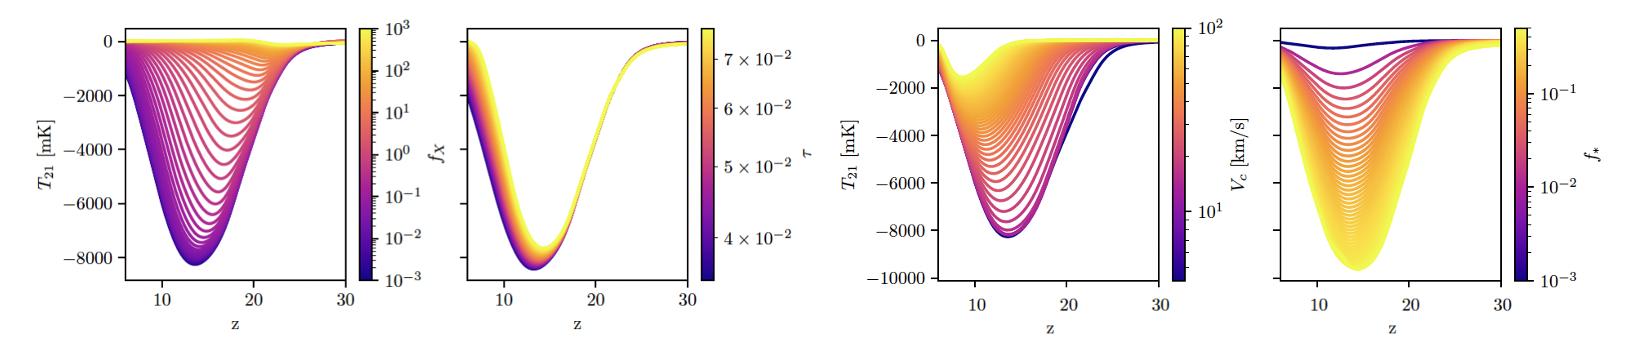
\includegraphics[width=1\textwidth]{Figures/bevins_emu_2023.png}
\tiny Figure from Bevins (2023).
\end{figure}
\end{center}

\end{frame}

\begin{frame}{Parametrised Forward Model}

% ------------------ TOP HALF ------------------
\vspace{-1em}
\begin{columns}

% ---------- LEFT COLUMN ----------
\begin{column}{0.48\textwidth}
\vspace{-1.7em}
{
\setbeamercolor{block title}{fg=white,bg=red!75!black}
\setbeamercolor{block body}{bg=red!10}
\vspace{0.75cm}
\begin{block}{The Global 21\,cm Signal}
\small 
The astrophysical parameters - $\approx 7$ params
\(\theta\): 
\vspace{-0.25cm}
\large
\[
T_{21}(\nu \mid \theta)
\]
\vspace{-0.2cm}
\end{block}
}
\vspace{-0.1cm}
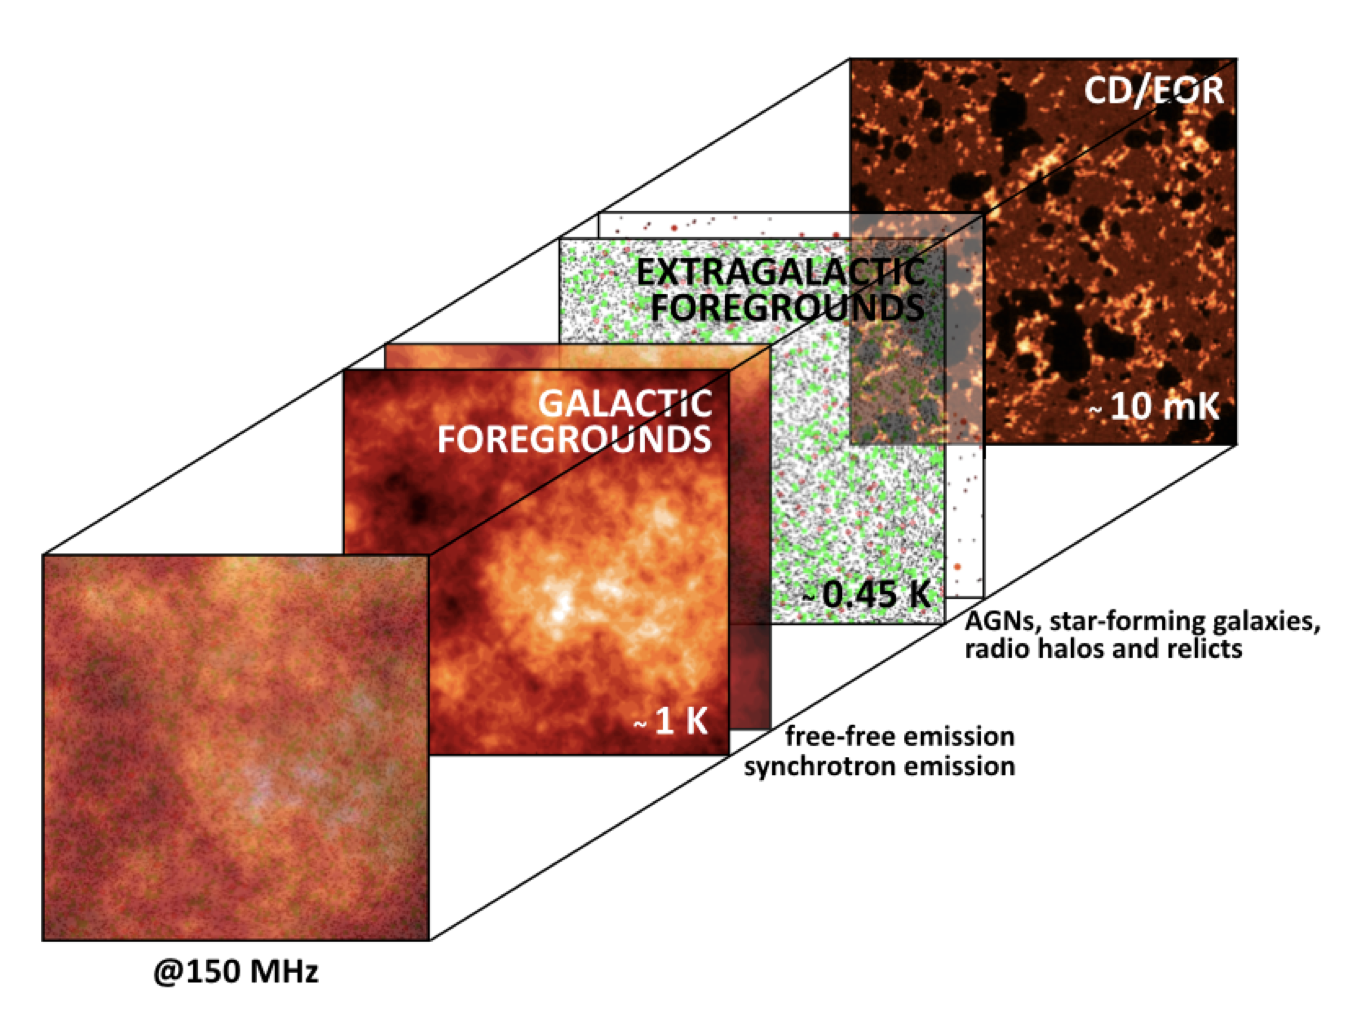
\includegraphics[width=0.9\textwidth]{Figures/foregrounds.png}
\vspace{-0.1cm}
\small
\tiny Figure from Chapman, Jelic (2019).
\end{column}
\begin{column}{0.48\textwidth}
\vspace{0.4em}
\begin{block}{The Galactic Foregrounds}
\small 
Model for the diffuse Galactic emission by splitting the sky into $N$ spectral-index regions, each parametised by
$\beta_i$ (Anstey et al 2021)
\end{block}

\vspace{0.3cm}
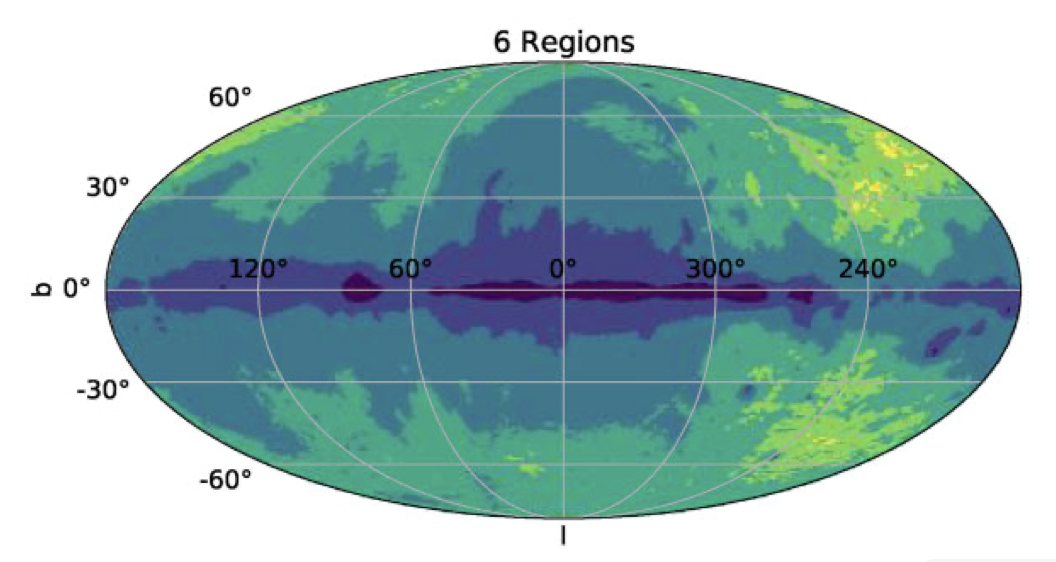
\includegraphics[width=0.98\textwidth]{Figures/spectral_mask.png}

\\[15pt]

\tiny Figure from Anstey et al (2021).

\end{column}
\end{columns}

\end{frame}

\begin{frame}{Parametrised Forward Model}

% ------------------ TOP HALF ------------------
\begin{columns}

% ---------- LEFT COLUMN ----------
\begin{column}{0.48\textwidth}
\vspace{-1em}
{
\setbeamercolor{block title}{fg=white,bg=red!75!black}
\setbeamercolor{block body}{bg=red!10}

\begin{block}{The Global 21\,cm Signal}
\vspace{0.4em}
\small 
The astrophysical parameters - $\approx 7$ params
\(\theta_{21}\): 

\large
\[
T_{21}(\nu \mid \theta)
\]

\end{block}
}

\begin{block}{The Hot Horizon}
\small 
Modeling an emissive and reflective horizon around the REACH telescope requiring parameterising soil temperature $T_{soil}$ and reflection coeff $|\Gamma|$. (Pattison et al 2024)

\end{block}



\end{column}

\begin{column}{0.48\textwidth}
\vspace{-1.1em}
\begin{block}{The Galactic Foregrounds}
\small 
Physics-motivated model for the diffuse Galactic emission $\approx 15 - 65$ params \(\theta_{for}\): 
\vspace{-1em}
\large
\[
T_{sky}(\nu \mid \theta)
\]
\vspace{-1.2em}
\end{block}
\centering
\vspace{0.7em}
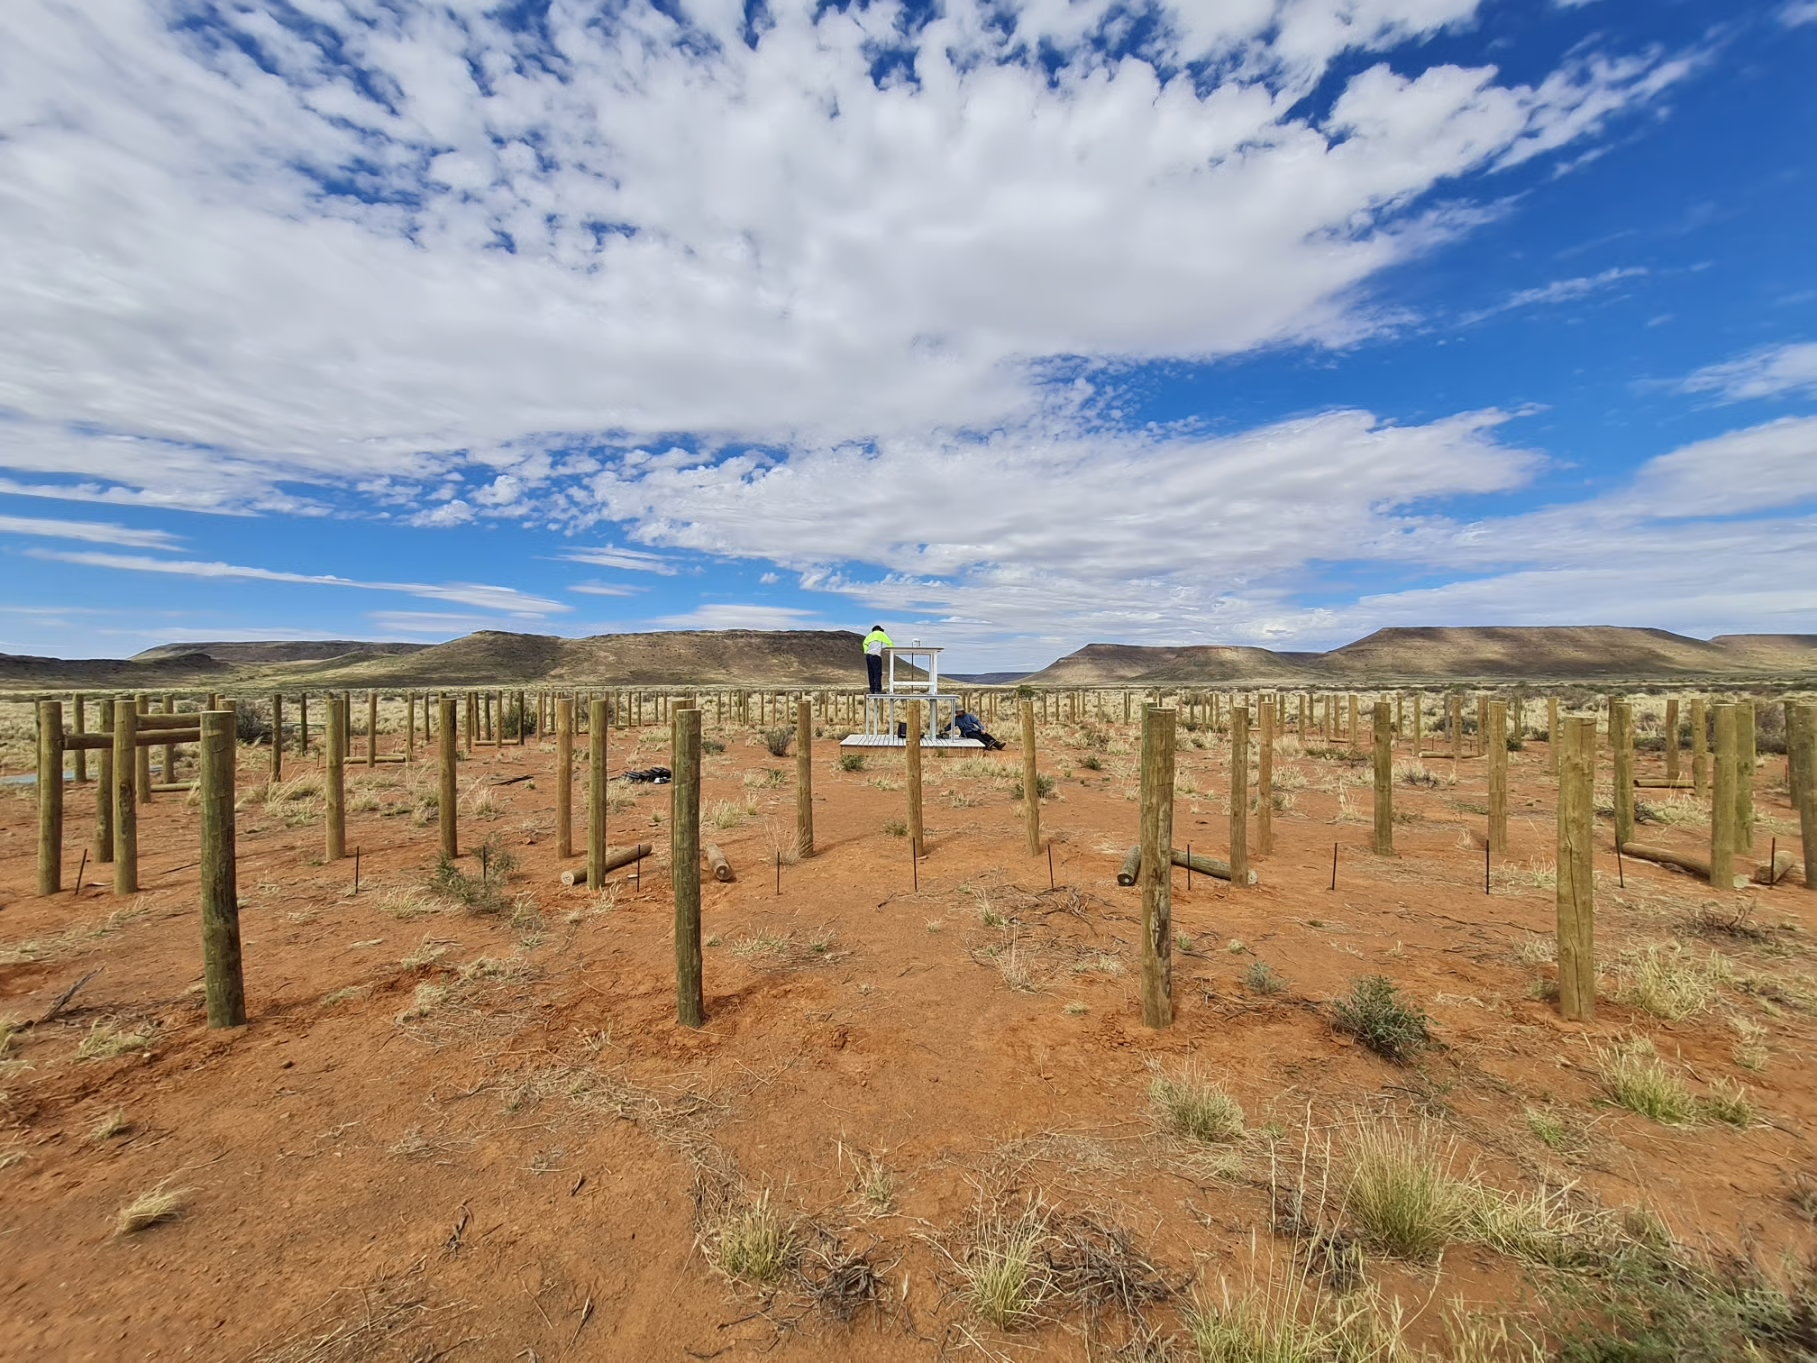
\includegraphics[width=\textwidth, trim=0 220 0 220, clip]{Figures/horizon.png}


\end{column}
\end{columns}

\end{frame}

\begin{frame}{Parametrised Forward Model}

% ------------------ TOP HALF ------------------
\begin{columns}

% ---------- LEFT COLUMN ----------
\begin{column}{0.49\textwidth}
\vspace{-1.5em}
{
\setbeamercolor{block title}{fg=white,bg=red!75!black}
\setbeamercolor{block body}{bg=red!10}

\begin{block}{The Global 21\,cm Signal}
\vspace{0.4em}
\small 
The astrophysical parameters - $\approx 7$ params
\(\theta_{21}\): 

\large
\[
T_{21}(\nu \mid \theta)
\]

\end{block}
}

\begin{block}{The Hot Horizon}
\small 
Modeling an emissive and reflective horizon around the REACH telescope requiring 2 extra params: $T_{soil}$ and $|\Gamma|$.
\vspace{2em}
\end{block}

\end{column}

\begin{column}{0.49\textwidth}
\vspace{-1.55em}
\begin{block}{The Galactic Foregrounds}
\small 
Physics-motivated model for the diffuse Galactic emission $\approx 15 - 65$ regions / params \(\theta_{for}\): 
\large
\vspace{-0.5em}
\[
T_{sky}(\nu \mid \theta)
\]
\vspace{-1.5em}
\end{block}

\begin{block}{Likelihood / Noise Structure}
\small
Different noise parameters
(\(\theta_{\mathrm{noise}}\)).  
{\tiny (Scheutwinkel, 2023)}
\vspace{-0.3em}
\scriptsize

\begin{itemize}
\item \textbf{Gaussian:} \(\theta_{\mathrm{noise}} = \{\sigma_L\}\)

\item \textbf{Generalised Normal:} \(\theta_{\mathrm{noise}} = \{\beta_L, \sigma_L\}\)

\item \textbf{Radiometric:} \(\theta_{\mathrm{noise}} = \{T_{\mathrm{rec}}, \eta, \sigma_{\mathrm{radio}}\}\)
\end{itemize}
\end{block}

\end{column}
\end{columns}
\end{frame}

\begin{frame}{Parametrised Forward Model}
\vspace{-1.9em}
% ------------------ TOP HALF ------------------
\begin{columns}

% ---------- LEFT COLUMN ----------
\begin{column}{0.49\textwidth}
\vspace{-1.5em}
{
\setbeamercolor{block title}{fg=white,bg=red!75!black}
\setbeamercolor{block body}{bg=red!10}

\begin{block}{The Global 21\,cm Signal}
\vspace{0.4em}
\small 
The astrophysical parameters - $\approx 7$ params
\(\theta_{21}\): 

\large
\[
T_{21}(\nu \mid \theta)
\]

\end{block}
}

\begin{block}{The Hot Horizon}
\small 
Modeling an emissive and reflective horizon around the REACH telescope requiring 2 extra params: $T_{soil}$ and $|\Gamma|$.
\vspace{2em}
\end{block}

\end{column}

\begin{column}{0.49\textwidth}
\vspace{-1.55em}
\begin{block}{The Galactic Foregrounds}
\small 
Physics-motivated model for the diffuse Galactic emission $\approx 15 - 65$ regions / params \(\theta_{for}\): 
\large
\vspace{-0.5em}
\[
T_{sky}(\nu \mid \theta)
\]
\vspace{-1.5em}
\end{block}

\begin{block}{Likelihood / Noise Structure}
\small
Different noise parameters
(\(\theta_{\mathrm{noise}}\)).  
{\tiny (Scheutwinkel, 2023)}
\vspace{-0.3em}
\scriptsize

\begin{itemize}
\item \textbf{Gaussian:} \(\theta_{\mathrm{noise}} = \{\sigma_L\}\)

\item \textbf{Generalised Normal:} \(\theta_{\mathrm{noise}} = \{\beta_L, \sigma_L\}\)

\item \textbf{Radiometric:} \(\theta_{\mathrm{noise}} = \{T_{\mathrm{rec}}, \eta, \sigma_{\mathrm{radio}}\}\)
\end{itemize}
\end{block}

\end{column}
\end{columns}

\vspace{-14em}
\begin{center}
\setbeamercolor{myredbox}{bg=red!20, fg=black}
\begin{beamercolorbox}[
    wd=\textwidth,
    rounded=true,
    shadow=true,
    sep=1em
]{myredbox}

And More:\\[5pt]
\begin{itemize}
    \item RFI Flagging (D Anstey and S Leeney, 2024)
    \item Extra-galactic Point Sources (S Mittal et al 2024)
    \item Forground Map Errors (M Pagona et al 2024)
\end{itemize}
\end{beamercolorbox}


\end{center}
\end{frame}



\begin{frame}{High-Dimensional Inference}
\vspace{-0.6em}
\footnotesize
\begin{block}{Typical analyses involve $30\!-\!80$ parameters:}
\vspace{-0.4em}
\begin{columns}[T]

% ---------- LEFT ----------
\begin{column}{0.48\textwidth}
\begin{itemize}
    \item $\sim 7$ astrophysical 
    \item $\sim 15\!-\!65$ foreground 
\end{itemize}
\end{column}

% ---------- RIGHT ----------
\begin{column}{0.48\textwidth}
\begin{itemize}
    \item $\sim 2$ horizon 
    \item $\sim 1\!-\!3$ noise 
\end{itemize}
\end{column}

\end{columns}
\end{block}

\textbf{$\Rightarrow$ millions of likelihood calls, $\sim$1-20 hours per run on CPUs.}

\pause

\vspace{0.5em}

\hrulefill

\vspace{0.5em}

\footnotesize
Using:

- {\color{red}\textbf{Chromatic functions} $K_{i,j,k}, R_{i,j,k}, J_i$}: (encode beam + instrument response)

- {\color{red}\textbf{Neural network emulator} $T_S(\nu,\theta_S)$} (fast 21-cm signal generation)

\tiny
\vspace{-0.6em}

% ------------------ LIKELIHOOD ------------------
\[
\log \mathcal{L}
=
\sum_{i,j}
\left[
-\tfrac{1}{2}\log\!\left(2\pi\,\theta_\sigma^2\right)
-
\tfrac{1}{2}
\left(
\frac{
T_D(\nu,t)
-
\left( T_F(\nu,t,\theta_F) 
      + {\color{red}T_S(\nu,\theta_S)}
\right)
}{
\theta_\sigma
}
\right)^2
\right]
\]

% ------------------ FORWARD MODEL ------------------

\[
T_{F_{i,j}}
=
\sum_k {\color{red}K_{i,j,k}}\, F_i(\theta_{F_k})
+
\sum_k {\color{red}R_{i,j,k}}\, F_i(\theta_{F_k})\,|\Gamma| \alpha
+
{\color{red}J_i}\, T_H\, (1 + |\Gamma| \alpha)
\]
\vspace{-0.2em}
\hfill \tiny{Credit: Pattison et al 2025}


\footnotesize
Inference reduces to {\color{red}\textbf{matrix multiplications + vector operations}}.

\hspace{1.5em}$\Rightarrow$ Ideally suited to the {\color{red}\textbf{SIMD/SIMT architecture of modern GPUs}}.

\pause
\vspace{-10em}
\begin{center}
\setbeamercolor{myredbox}{bg=red!20, fg=black}
\begin{beamercolorbox}[
    wd=\textwidth,
    rounded=true,
    shadow=true,
    sep=1em
]{myredbox}
\centering
\large
\textbf{To allow wider time ranges and higher-dim models: \\[5pt]
Our pipelines must move to GPU-accelerated inference.}
\end{beamercolorbox}
\end{center}
\end{frame}


\begin{frame}{Modern Computational Architecture}
\vspace{-0.4em}
% ----- LEFT: CPU -----
\begin{block}{CPU Architecture}
\begin{columns}
\begin{column}{0.65\textwidth}
\vspace{-0.3em}
\begin{itemize}\small
    \item Few powerful cores (10s)
    \item Complex control logic
    \item Optimised for sequential workloads
    \item Large caches, low latency
\end{itemize}
\end{column}
\begin{column}{0.28\textwidth}
\vspace{-0.3em}
\begin{center}
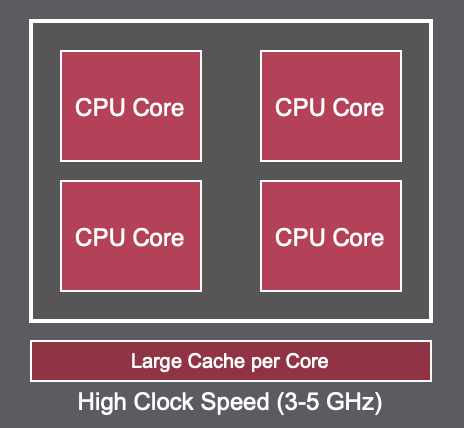
\includegraphics[width=0.8\linewidth]{Figures/cpustructure.png}
\end{center}
\end{column}
\end{columns}
\end{block}

\vspace{-0.4em}
% ----- RIGHT: GPU -----
{
\setbeamercolor{block title}{fg=white,bg=red!75!black}
\setbeamercolor{block body}{bg=red!10}
\begin{block}{GPU Architecture}
\begin{columns}
\begin{column}{0.28\textwidth}
\vspace{-0.4em}
\begin{center}
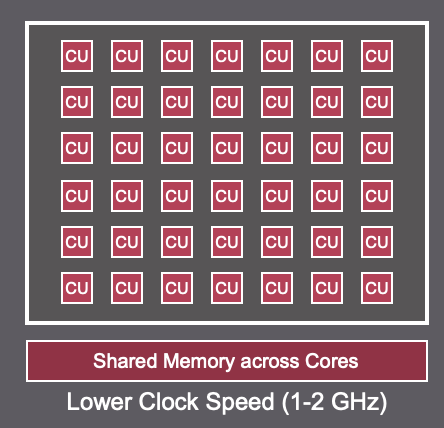
\includegraphics[width=0.8\linewidth]{Figures/GPUstructure.png}
\end{center}
\end{column}

\begin{column}{0.65\textwidth}
\vspace{-0.4em}
\begin{itemize}\small
    \item Thousands of lightweight cores
    \item Massive parallelism (SIMT)
    \item High memory bandwidth
    \item Excel at batched vectorised operations
\end{itemize}
\end{column}
\end{columns}
\hfill \tiny{Image Credit: AMD}
\end{block}
}
\end{frame}
\begin{frame}{An Introduction to JAX}
\footnotesize
% ---------------- TOP BAR ----------------
\begin{columns}[T,totalwidth=\textwidth]

% ---- LEFT: JAX logo + subtitle ----
\begin{column}{0.28\textwidth}
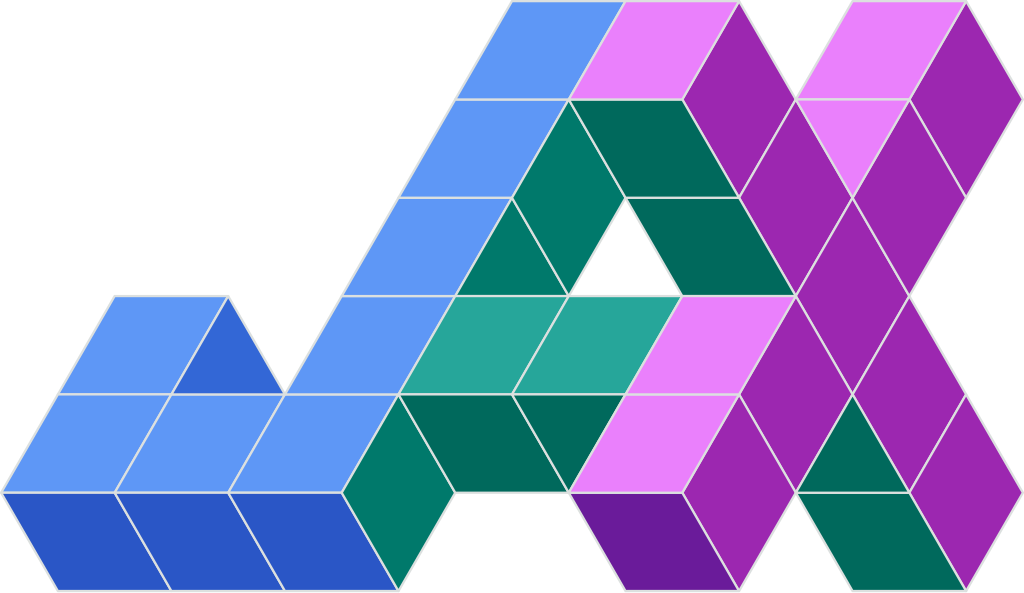
\includegraphics[width=0.75\linewidth]{Figures/jax.png}

\vspace{0.2em}
\footnotesize
\textbf{High-performance numerical-computing}\\
\textbf{and large-scale machine learning}
\end{column}
\pause
\begin{column}{0.715\textwidth}
\vspace{-1.4em}
\begin{block}{Automatic Differentiation}
\vspace{-0.6em}
\small
\[
(\nabla f)(x)_i = \frac{\partial f}{\partial x_i}(x)
\quad\Longrightarrow\quad 
\texttt{jax.grad(f)(x)}
\]
\scriptsize For more details on Autodiff/Dual Numbers see \\ \faGithub\ \href{https://github.com/JacobTutt/dual_autodiff_package}{JacobTutt/dual\_autodiff\_package}
\vspace{-0.3em}
\end{block}
\pause 

\vspace{-0.8em}
\begin{block}{XLA Compilation}
\vspace{-0.5em}
\small
\scriptsize
\begin{itemize}
    \item Transforms functions into optimised machine code
    \item Provides python flexibility alongside compiled language preformance
\end{itemize}

\vspace{-1.5em}
\[
f(x) \quad\Longrightarrow\quad \texttt{jax.jit}(f)(x)
\]
\vspace{-1em}
\end{block}
\pause 
\vspace{-0.7em}
\begin{block}{Automatic Vectorisation and Parallelisation}
\small
\vspace{-0.8em}
\begin{itemize}\scriptsize
    \item \textbf{\texttt{jax.vmap}}: automatic vectorisation over batches of data  

    \item \textbf{\texttt{jax.pmap}}: parallel execution across multiple XLA devices  
\end{itemize}
\vspace{-0.3em}
\end{block}
\end{column}
\end{columns}
\end{frame}

\begin{frame}{Benchmarking Performance Increases}
\textbf{Data/ Chromaticity Function Generation}
\medskip
\scriptsize
\begin{enumerate}

  \item \textbf{Foreground model} \\
        Build $T_{\rm sky}(\Omega,\nu)$ with base + spectral index maps
        (power-law scaling around $\nu_0$).
        
  \item \textbf{Galactic Transforms} \\
        Transform maps from Galactic to Local (AltAz) frames

  \item \textbf{Lunar / horizon environment} \\
        Inject lunar emission and horizon + soil emission/reflection model.

  \item \textbf{Antenna convolution} \\
        Apply chromatic antenna pattern
        $A(\nu,\Omega)$, and average over the sky:
        $T_{\rm ant}(\nu,t)$.

  \item \textbf{Time reduction} \\
        Optionally collapse time dimension (Averaged vs Separated).

  \item \textbf{Noise model} \\
        Add instrumental noise using the selected
        model (Gaussian, radiometric, etc.).

  \item \textbf{21-cm signal injection} \\
        Add the cosmological global signal model $T_{21}(\nu)$.

\end{enumerate}
\end{frame}


\begin{frame}{Benchmarking Performance Increases}


\textbf{Data Generation Pipeline}
\footnotesize
\begin{itemize}
    \item Computed for 13 time intervals
\end{itemize}
\vspace{-1.2em}

\begin{columns} 
% ---------- LEFT COLUMN: TABLE ----------
\begin{column}{0.45\textwidth}
\footnotesize
\begin{table}[h]
\centering
\footnotesize
\begin{tabular}{lcc}
\hline
\textbf{Configuration} & \textbf{Old (s)} & \textbf{New (s)} \\
\hline
Ave No Horizon      & 661 & 50 \\
Ave Horizon         & 655 & 50 \\
Sep No Horizon     & 725 & 52 \\
Sep Horizon        & 813 & 53 \\
\hline
\end{tabular}

\vspace{0.4em}
\raggedright 
{\tiny
\emph{* Old pipeline - 40-core CPU node (\£0.40/hr)\\ 
* New pipeline - NVIDIA A100 GPU(\£0.55/hr)\\}
}
\end{table}
\end{column}

% ---------- RIGHT COLUMN: IMAGE ----------
\begin{column}{0.53\textwidth}
\begin{figure}
\centering
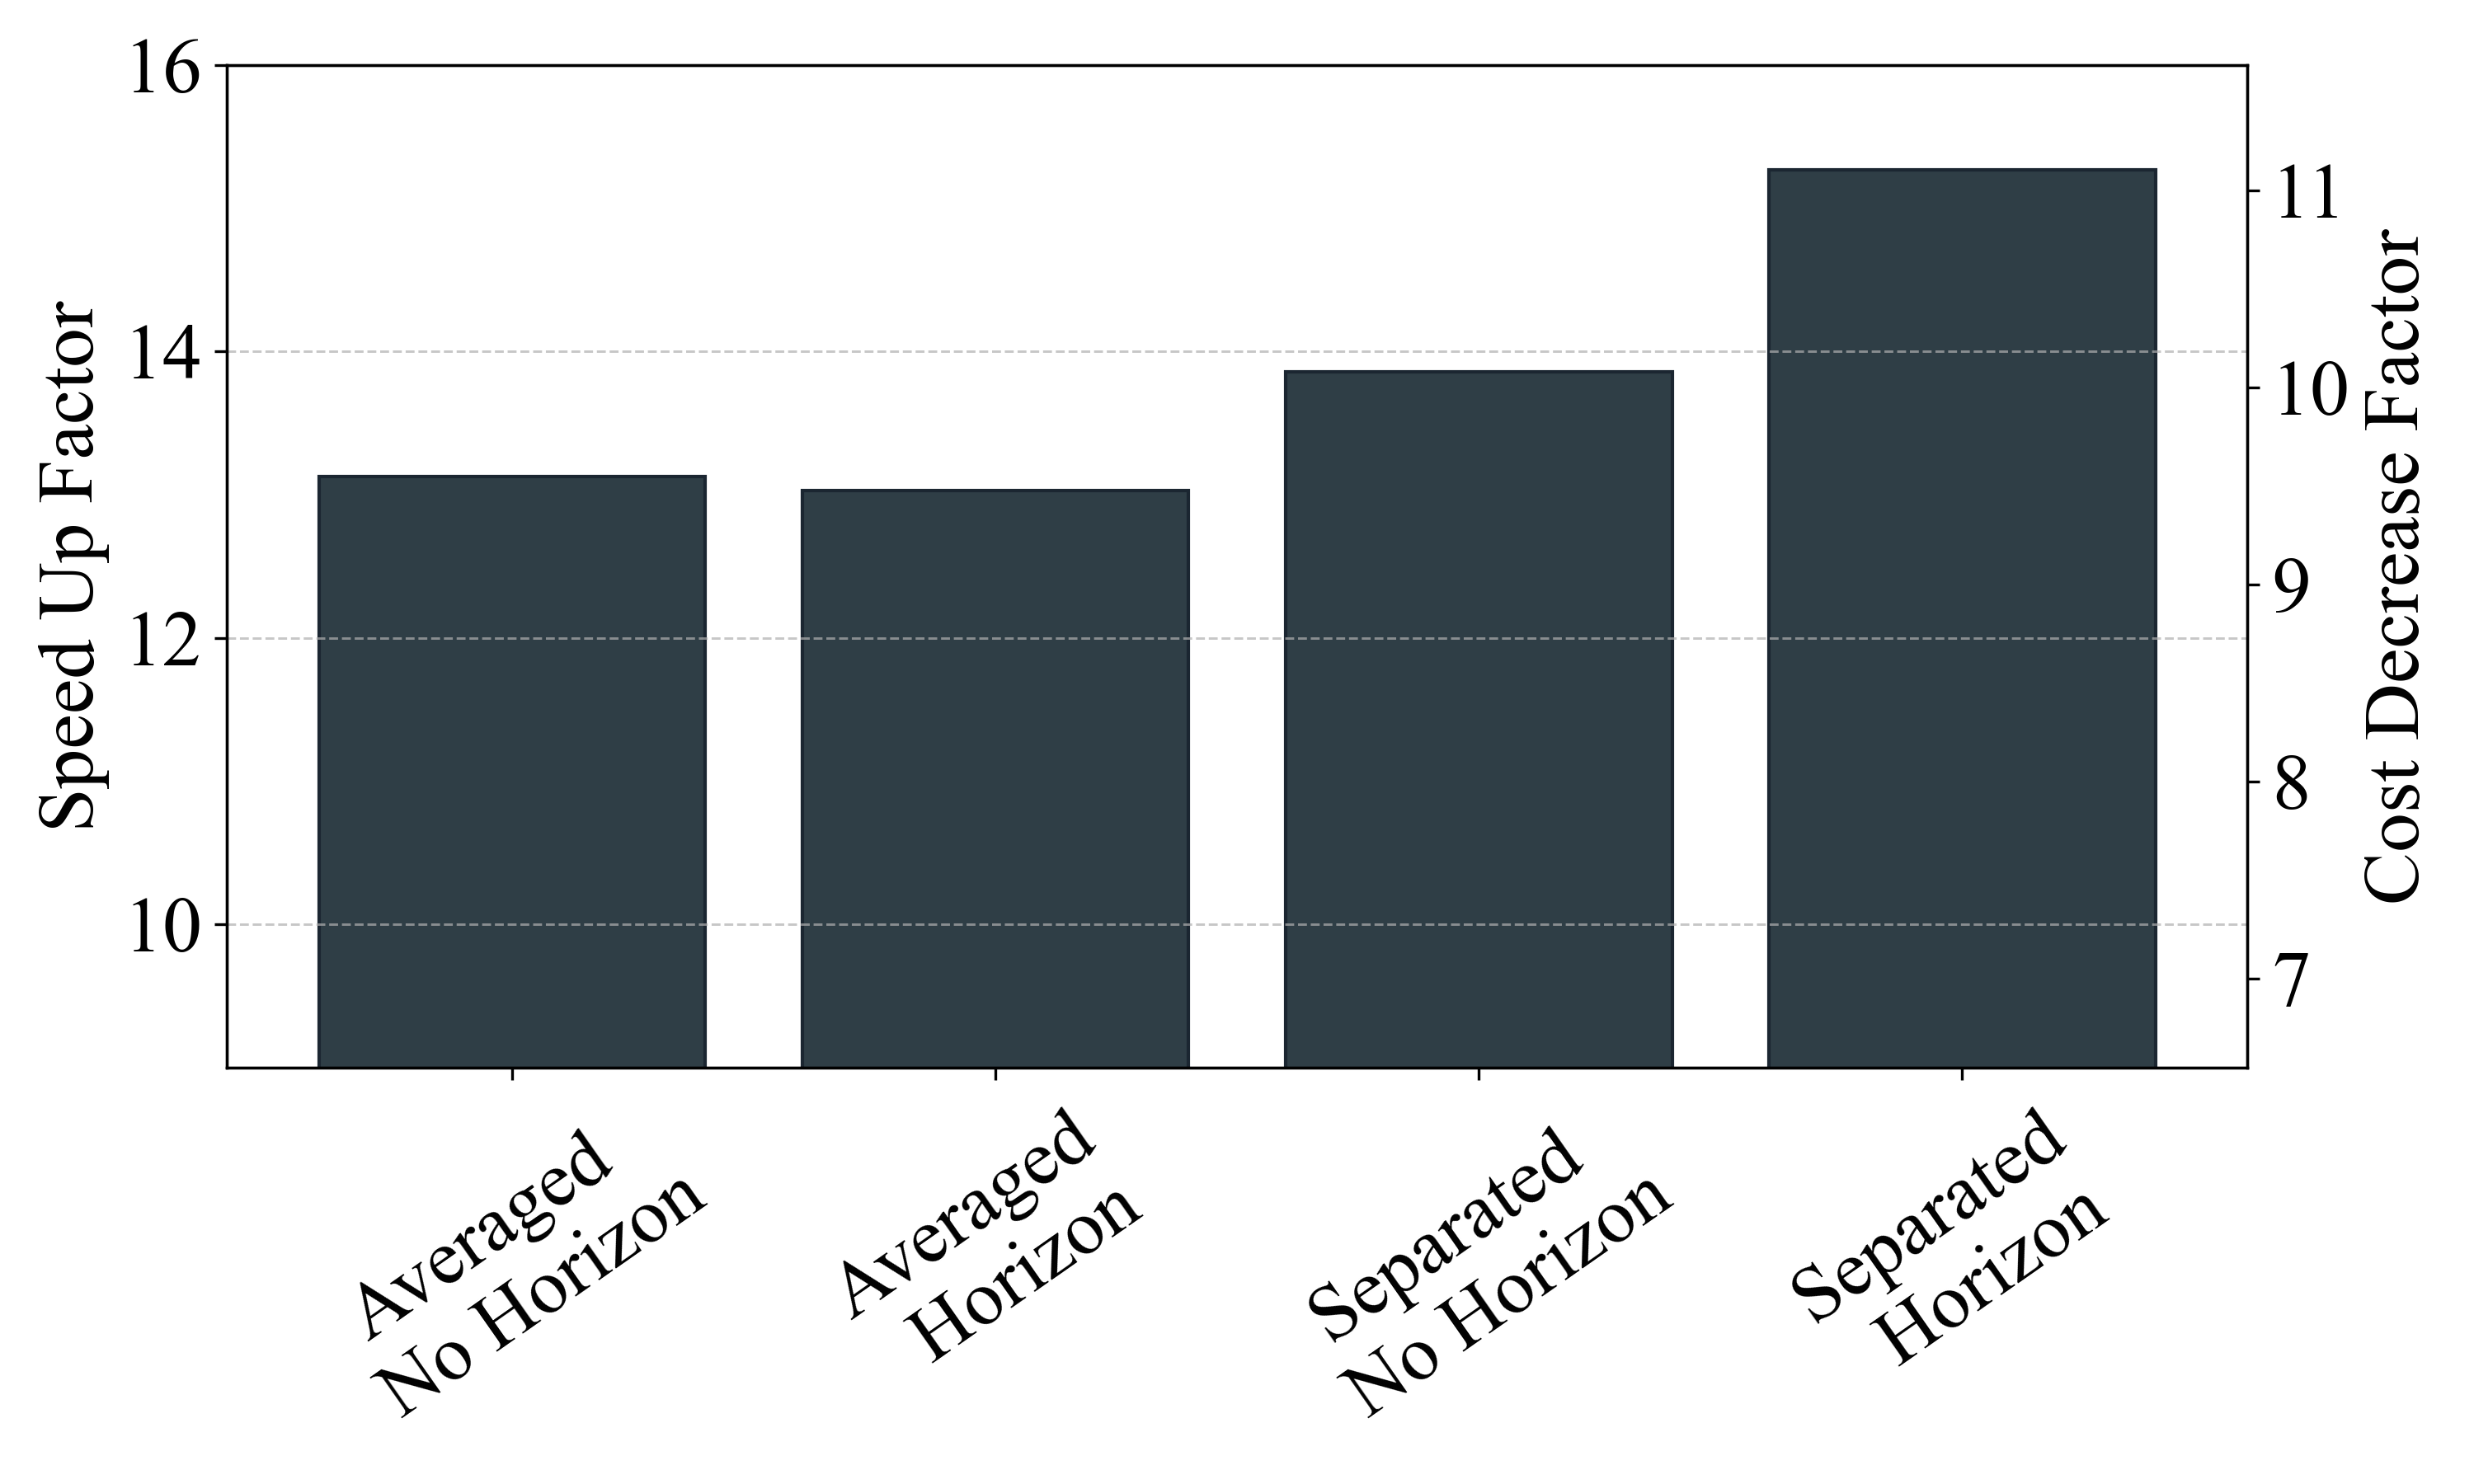
\includegraphics[width=\linewidth]{Figures/datagen_comparison.png}
\end{figure}
\end{column}

\end{columns}
\footnotesize
\raggedright
{\textbf{Key Takeaway:} Speed up of up to \textbf{15X} \\ \hspace{64pt} (11X Financial Saving)}

\end{frame}


\begin{frame}{Benchmarking Performance Increases}

\textbf{Chromaticity Function Generation}
\footnotesize
\begin{itemize}
    \item Computed for 13 time intervals and 35 regions
\end{itemize}
\vspace{-1.2em}
\begin{columns} 

% ---------- LEFT COLUMN: TABLE ----------
\begin{column}{0.45\textwidth}
\footnotesize
\begin{table}[h]
\centering
\footnotesize
\begin{tabular}{lcc}
\hline
\textbf{Configuration} & \textbf{Old (s)} & \textbf{New (s)} \\
\hline
Ave No Horizon      & 328 & 51 \\
Ave Horizon         & 406 & 52 \\
Sep No Horizon     & 1474 & 53 \\
Sep Horizon        & 2326 & 54 \\
\hline
\end{tabular}

\vspace{0.4em}
\raggedright 
{\tiny
\emph{* Old pipeline - 40-core CPU node (\£0.40/hr)\\ 
* New pipeline - NVIDIA A100 GPU(\£0.55/hr)\\}
}
\end{table}
\end{column}

% ---------- RIGHT COLUMN: IMAGE ----------
\begin{column}{0.53\textwidth}
\begin{figure}
\centering
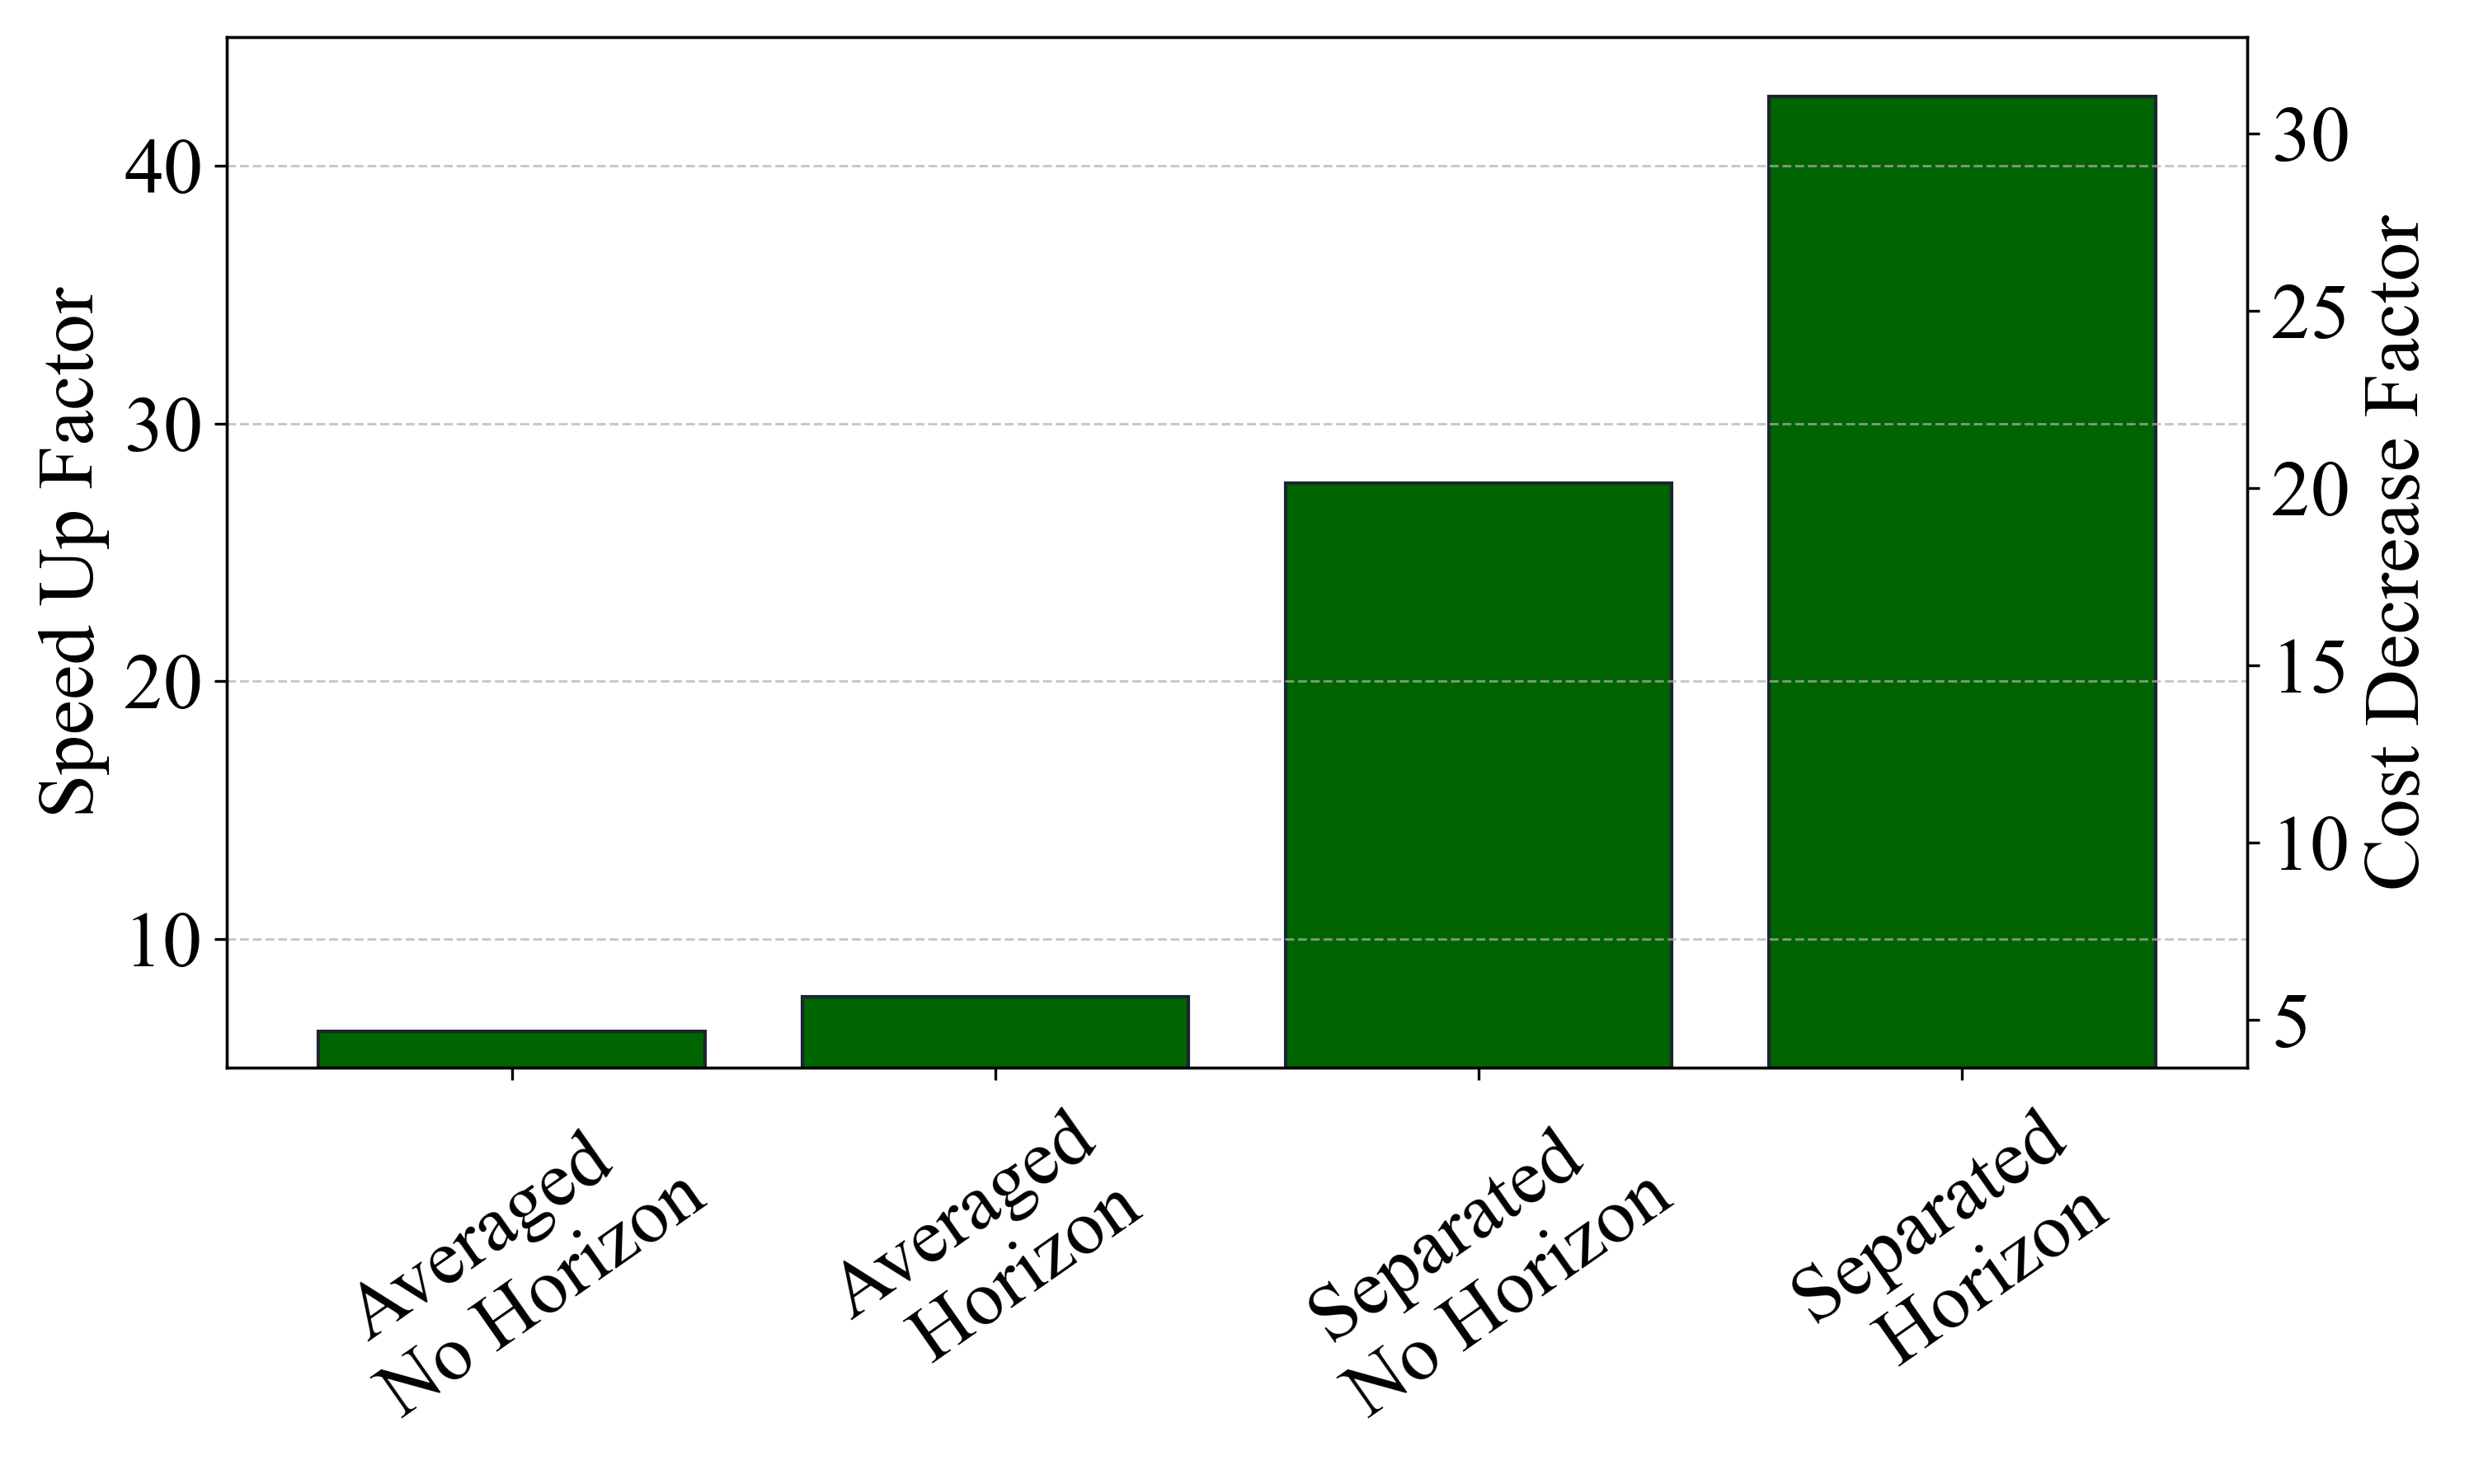
\includegraphics[width=\linewidth]{Figures/chromfunc_comparison.png}
\end{figure}
\end{column}
\end{columns}
\raggedright
{\textbf{Key Takeaway:} Speed up of up to \textbf{43X} \\ \hspace{64pt} (31X Financial Saving)}

\end{frame}

\begin{frame}{Benchmarking Performance Increases}
\textbf{Data / Chromaticity Function Generation}

\medskip
\footnotesize
\begin{table}[h]
\centering
\renewcommand{\arraystretch}{1.2}
\begin{tabular}{l c}
\hline
\textbf{Pipeline Stage} & \textbf{Run Time} \\
\hline
\textcolor{red}{\textbf{Initialising/ Loading Data}}              & \textcolor{red}{$\sim\mathcal{O}(24s)$} \\
\textcolor{red}{\textbf{Galactic Transforms (CPU)}}       & \textcolor{red}{$\sim\mathcal{O}(26s)$} \\

\multirow{}{}{\textcolor{green!40!black}{\parbox{0.45\textwidth}{
\textbf{Spectral Index Broadcasting}\\
\textbf{Sky Map Interpolation}\\
\textbf{Lunar / Horizon Injection}\\
\textbf{Antenna Convolution}\\
\textbf{Time Averaging}\\
\textbf{Noise Model}\\
\textbf{21-cm Signal Injection}
}}}
& \textcolor{green!40!black}{$\sim\mathcal{O}(0.75s)$} \\
\hline
\end{tabular}
\end{table}
\end{frame}

\begin{frame}{Benchmarking Performance Increases}
\textbf{Individual Likelihood Call}
\footnotesize
\begin{itemize}
    \item Computed for 13 time intervals and 35 regions
\end{itemize}
\vspace{-1.4em}


\begin{columns} 

% ---------- LEFT COLUMN: TABLE ----------
\begin{column}{0.45\textwidth}
\footnotesize
\begin{table}[h]
\centering
\footnotesize
\begin{tabular}{lcc}
\hline
\textbf{Configuration} & \textbf{Old(ms)} & \textbf{New(ms)} \\
\hline
Ave No Horizon  & 0.31 & 0.08 \\
Ave Horizon   & 0.47 & 0.12 \\
Sep No Horizon  & 1.05 & 0.08 \\
Sep Horizon     & 2.80 & 0.13 \\
\hline
\end{tabular}

\vspace{0.4em}
\raggedright 
{\tiny
\emph{* Averaged Over 1000 Likelihood Calls\\
* Old pipeline - 40-core CPU node (\£0.40/hr)\\ 
* New pipeline - NVIDIA A100 GPU(\£0.55/hr)\\}
}
\end{table}
\end{column}

% ---------- RIGHT COLUMN: IMAGE ----------
\begin{column}{0.5\textwidth}
\begin{figure}
\centering
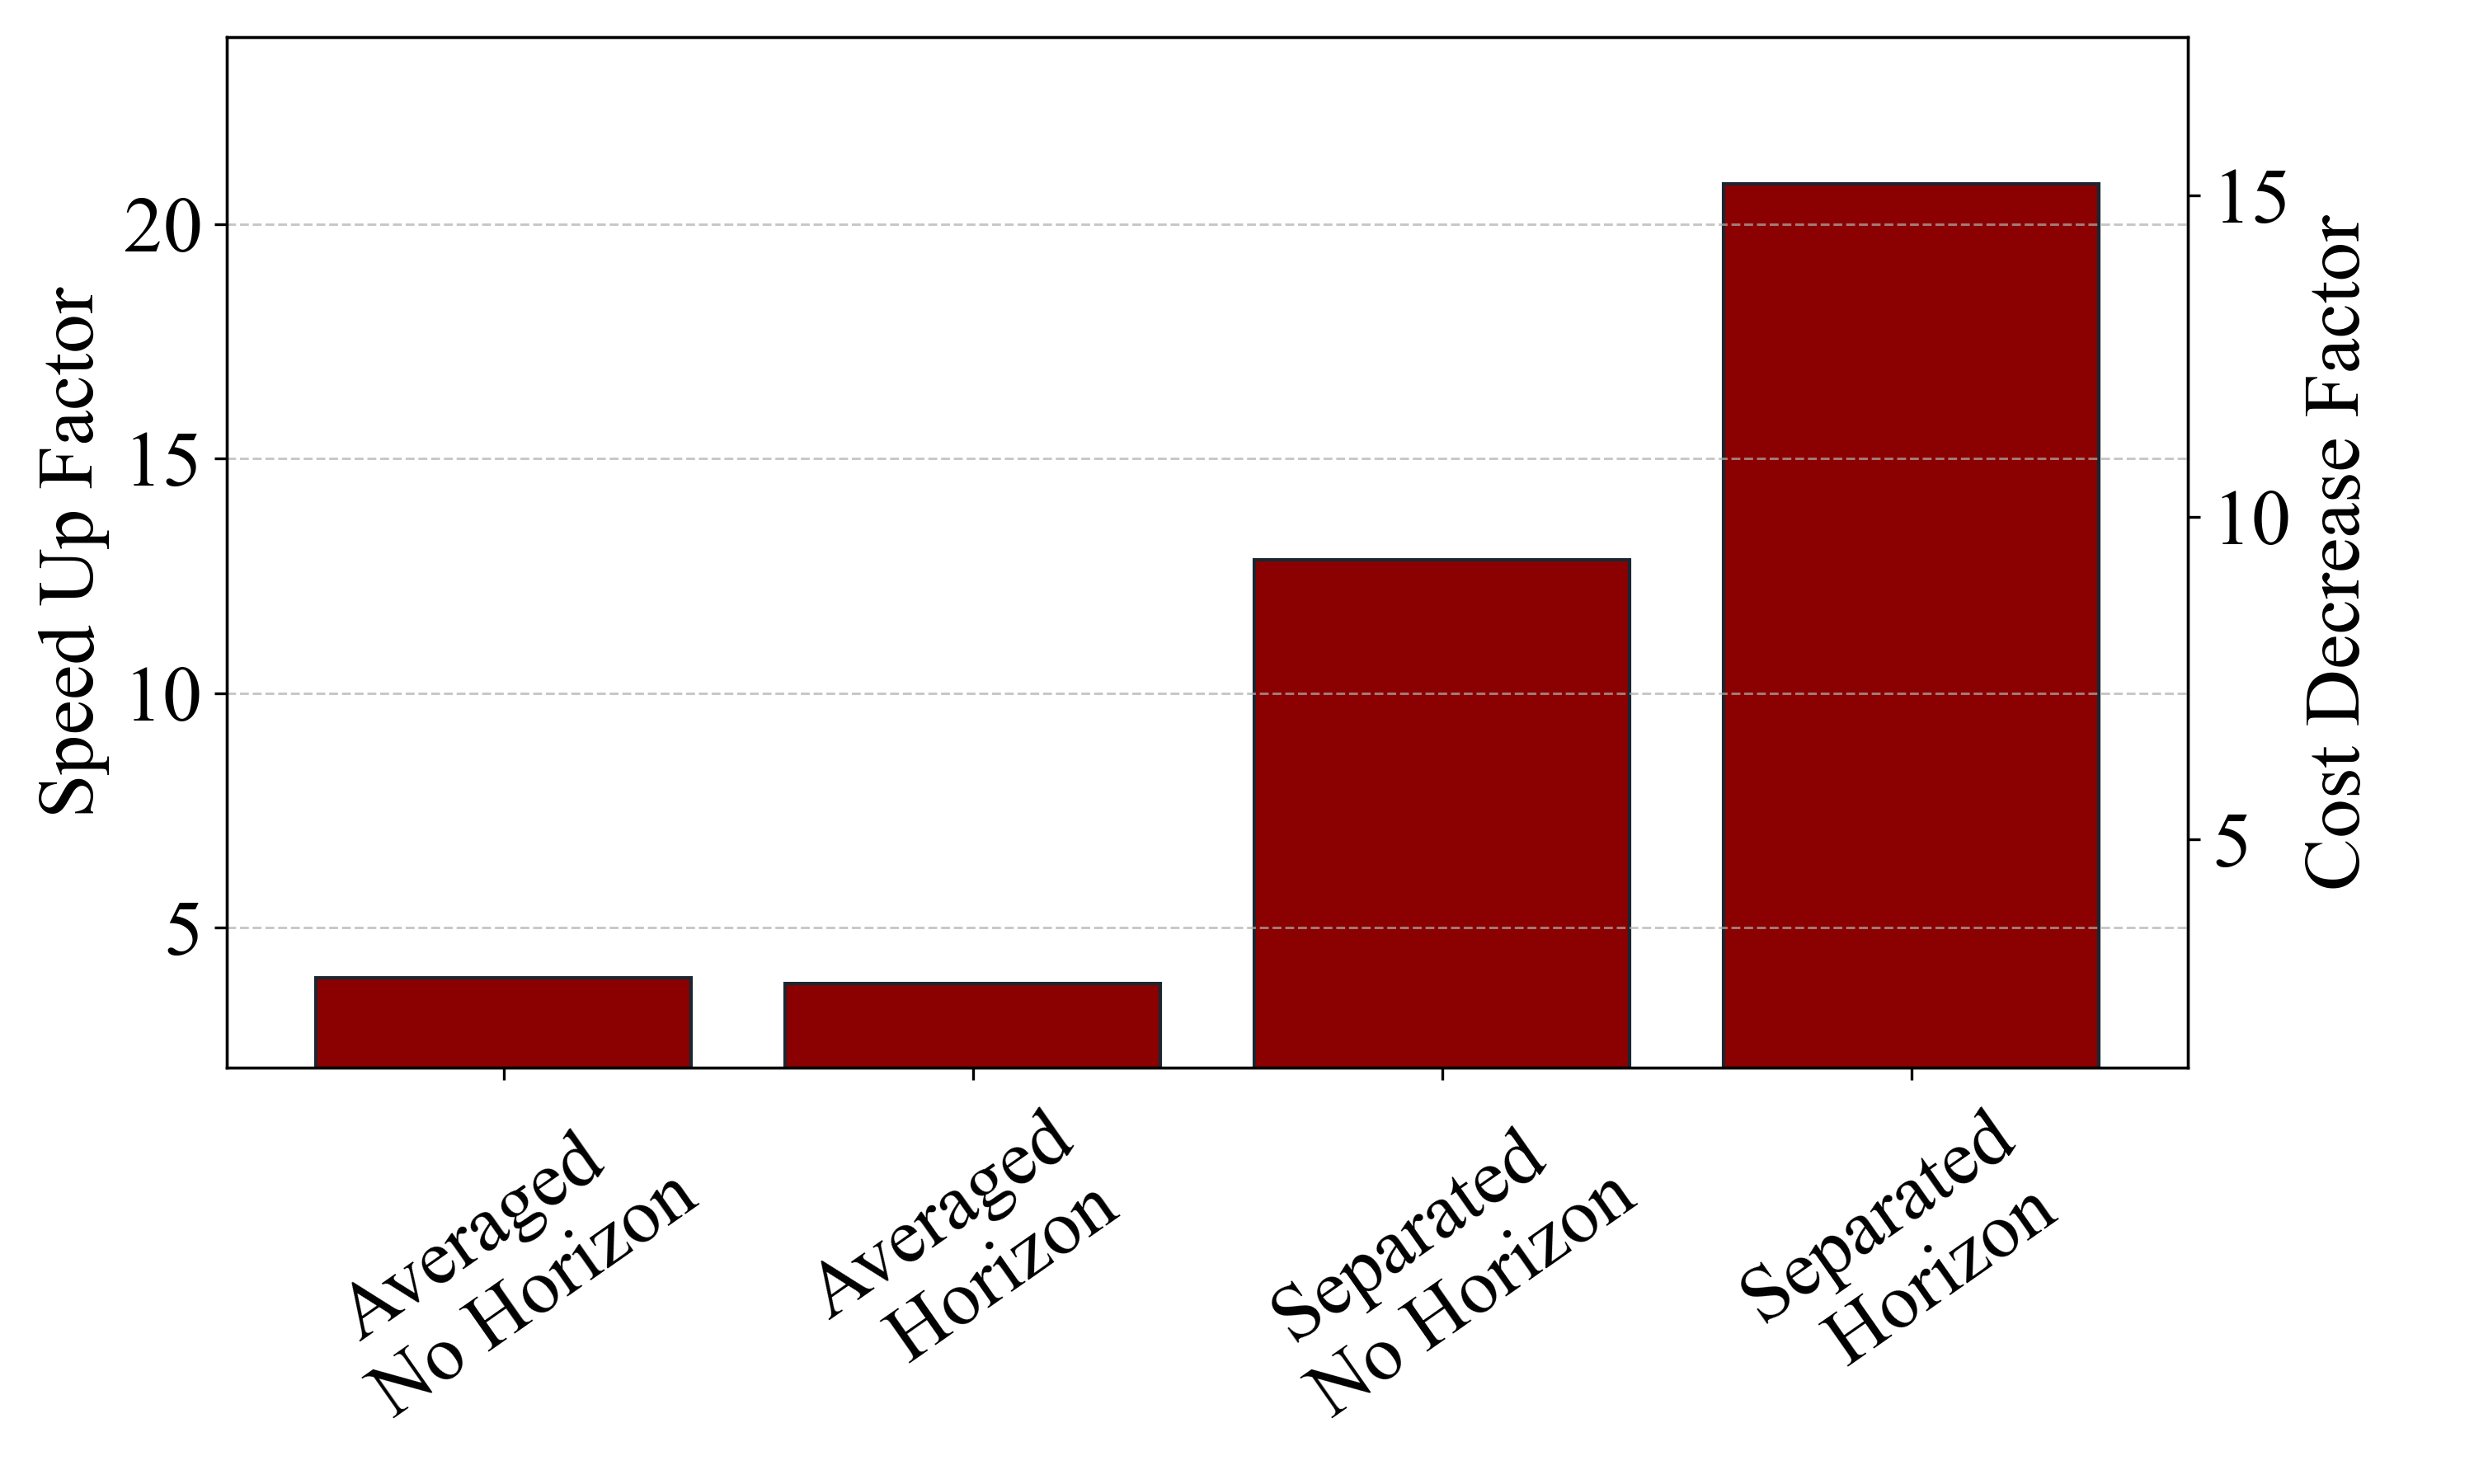
\includegraphics[width=1.1\linewidth]{Figures/like_comparison.png}
\end{figure}
\end{column}
\end{columns}
\raggedright
{\textbf{Key Takeaway:} Speed up of up to \textbf{21X} \\ \hspace{64pt} (15X Financial Saving)}
\end{frame}


\begin{frame}{Traditional Nested Sampling}
\vspace{-1.8em}
\begin{columns}
    % ---------- LEFT COLUMN ----------
    \begin{column}{0.60\textwidth}
    \scriptsize
    \textbf{Nested Sampling provides:}
    \begin{itemize}
        \item Posterior samples
        \item \textcolor{red}{\textbf{The Bayesian Evidence}} 
    \end{itemize}
    
    \tiny
    \textbf{Evidence integral:}
    \vspace{-1em}
    \[
    Z \;=\; \int_{\Theta} \mathcal{L}(\theta)\,\pi(\theta)\,d\theta
        \;=\; \int_{0}^{1} \mathcal{L}(\xi)\, d\xi .
    \]
    
    
    \textbf{Prior volume (mass):}
        \vspace{-1em}
    \[
    \xi(\mathcal{L}) \;=\; 
    \int_{\mathcal{L}(\theta) > \mathcal{L}} \pi(\theta)\, d\theta
    \qquad
    \Longrightarrow\quad
    \text{inverse relation: }\; \mathcal{L}(\xi)
    \]
    \vspace{-1em}
    \textbf{Shrinkage of the prior mass:}
    \[
    \xi_i = t \,\,\, \xi_{i-1},
    \]
    Expected shrinkage:
    \vspace{-2em}
    \[
    \mathbb{E}[log \, \, t] = - \frac{1}{N_{\text{live}}}
    \quad\Longrightarrow\quad
    \xi_i \approx \exp\!\left(-\frac{i}{N_{\text{live}}}\right)
    \]
    
    \vspace{-2em}
    \[
    \textcolor{red}{
    \boldsymbol{
    Z \;\approx\; \sum_i \mathcal{L}_i (\xi_{i-1} - \xi_i) =  \sum_i \mathcal{L}_i \Big[ \exp\!\left(-\frac{i-1}{N_{\text{live}}}\right) -  \exp\!\left(-\frac{i+1}{N_{\text{live}}}\right) \Big]}}
    \]
    
    \end{column}

    % ---------- RIGHT COLUMN ----------
    \begin{column}{0.325\textwidth}
        \vspace{1em}
        \begin{figure}
            \centering

            % ----------- SHOW IMAGE 1 ON OVERLAY 1 -----------
            \only<1>{
            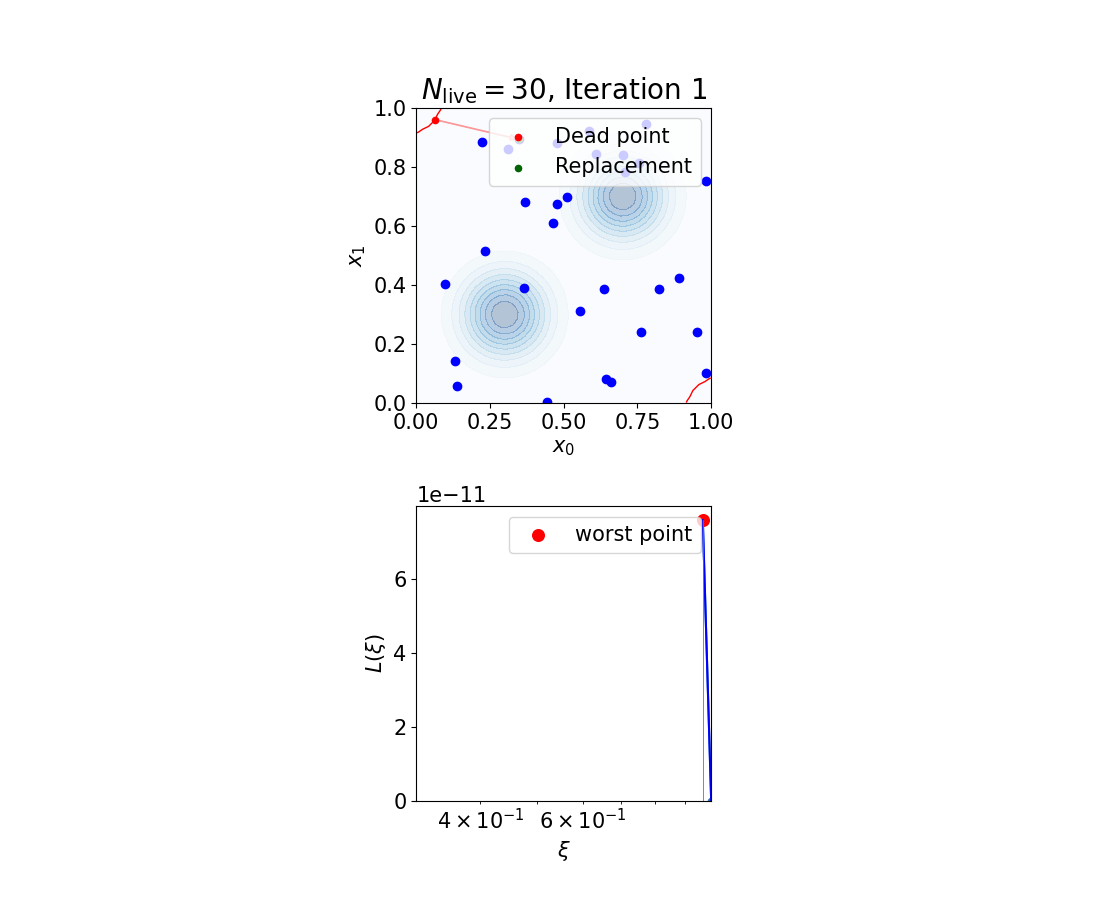
\includegraphics[width=\linewidth,
                             trim=240 20 250 50, clip]{Figures/NS/nested_sampling_1.png}
            }

            % ----------- SHOW IMAGE 10 ON OVERLAY 2 -----------
            \only<2>{
            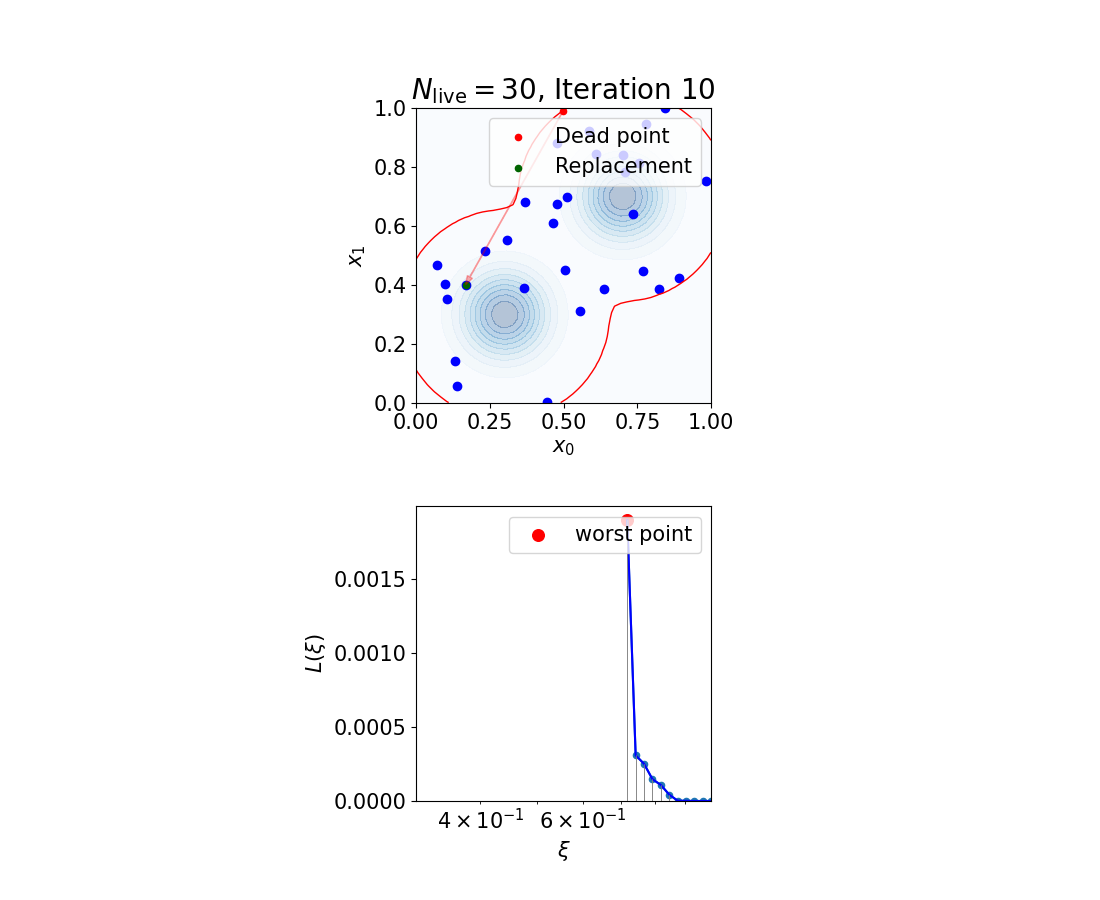
\includegraphics[width=\linewidth,
                             trim=240 20 250 50, clip]{Figures/NS/nested_sampling_10.png}
            }

            % ----------- SHOW IMAGE 30 ON OVERLAY 3 -----------
            \only<3>{
            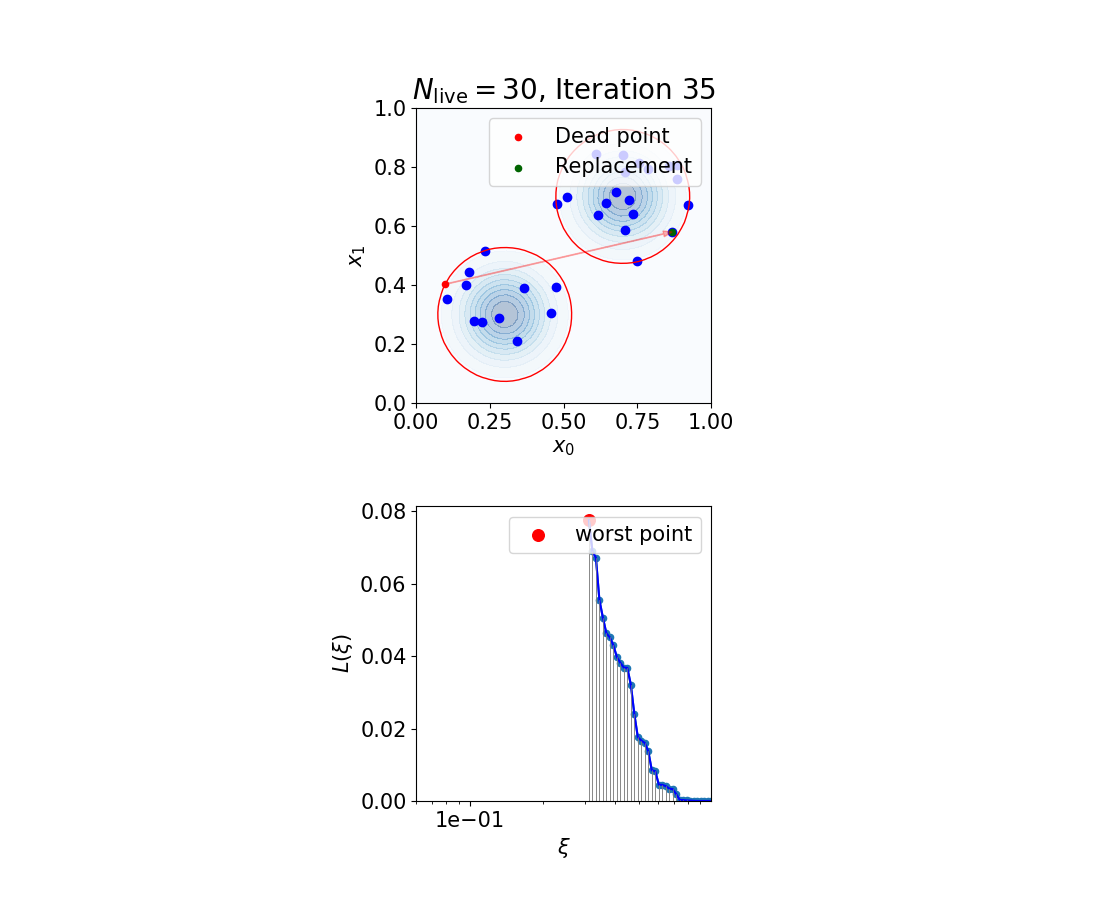
\includegraphics[width=\linewidth,
                             trim=240 20 250 50, clip]{Figures/NS/nested_sampling_35.png}
            }
            \only<4>{
            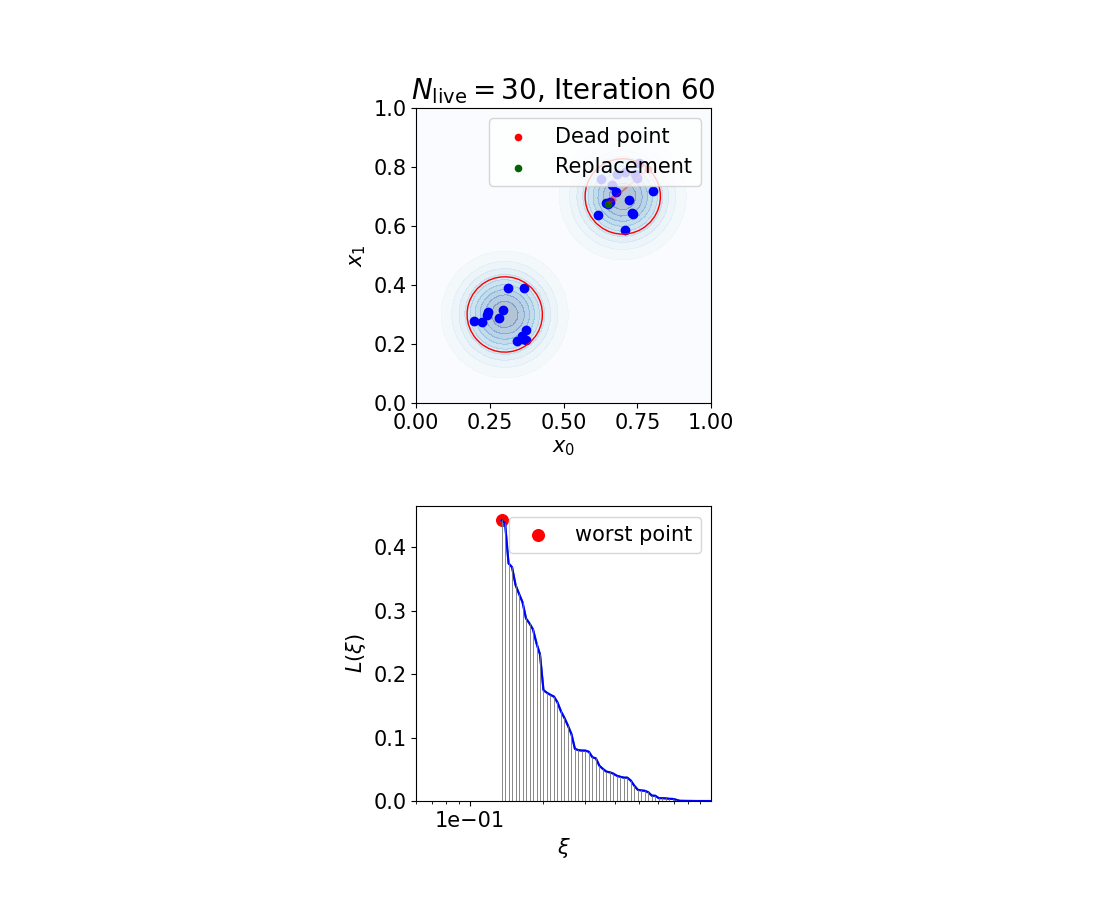
\includegraphics[width=\linewidth,
                             trim=240 20 250 50, clip]{Figures/NS/nested_sampling_60.png}
            }
            \only<5>{
            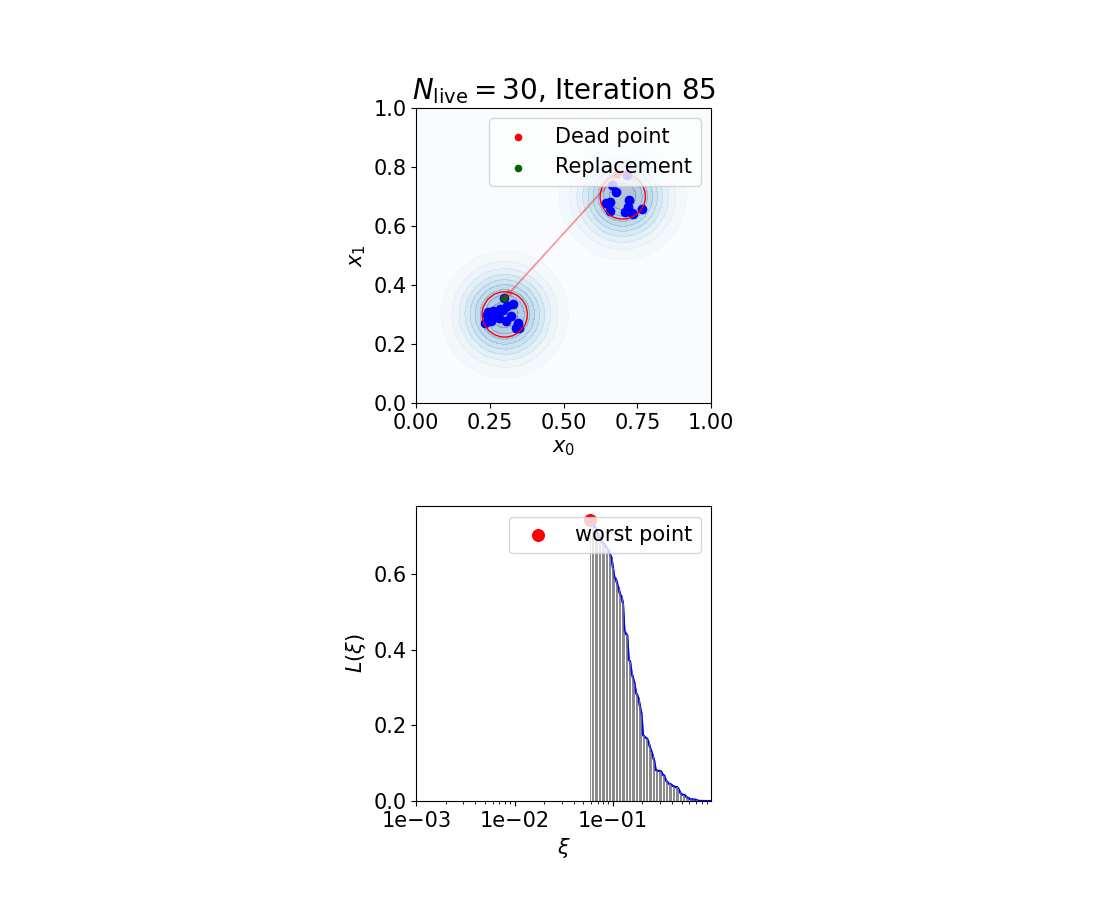
\includegraphics[width=\linewidth,
                             trim=240 20 250 50, clip]{Figures/NS/nested_sampling_85.png}
            }
            \only<6>{
            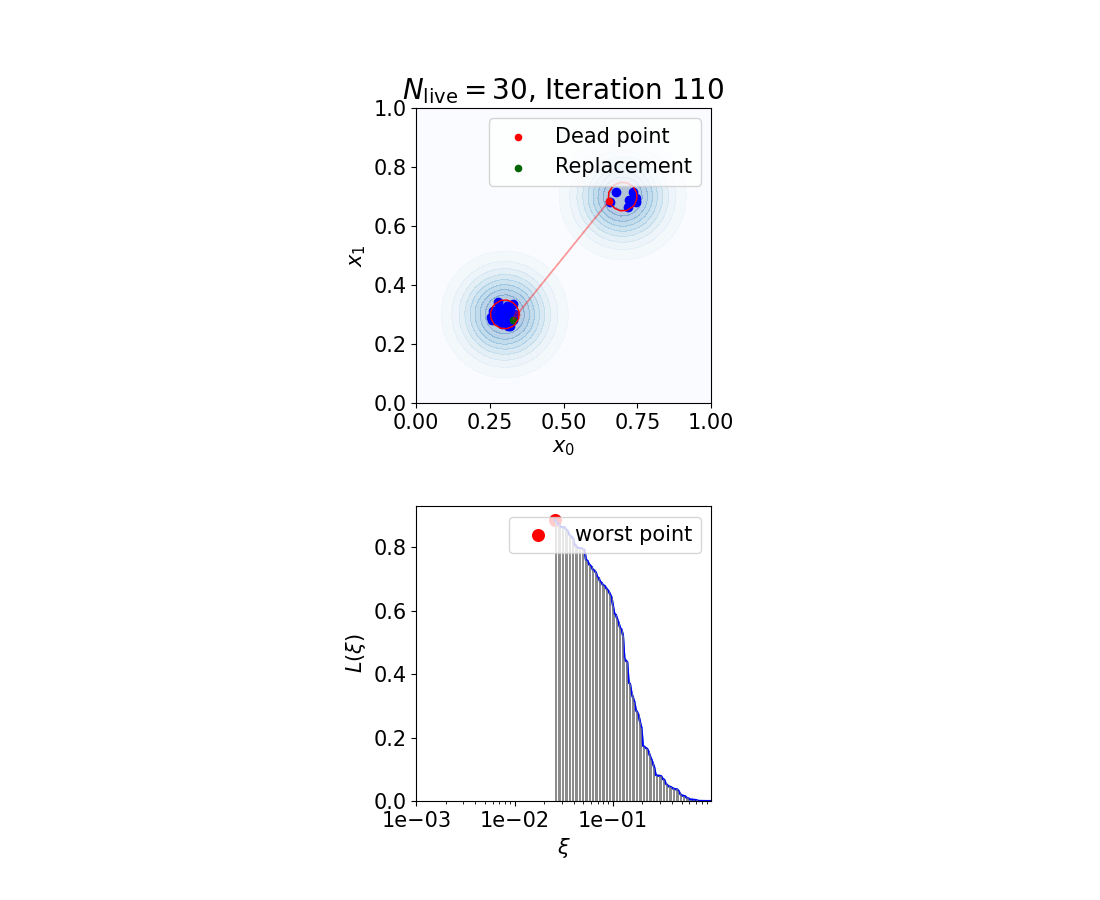
\includegraphics[width=\linewidth,
                             trim=240 20 250 50, clip]{Figures/NS/nested_sampling_110.png}
            }
            \only<7>{
            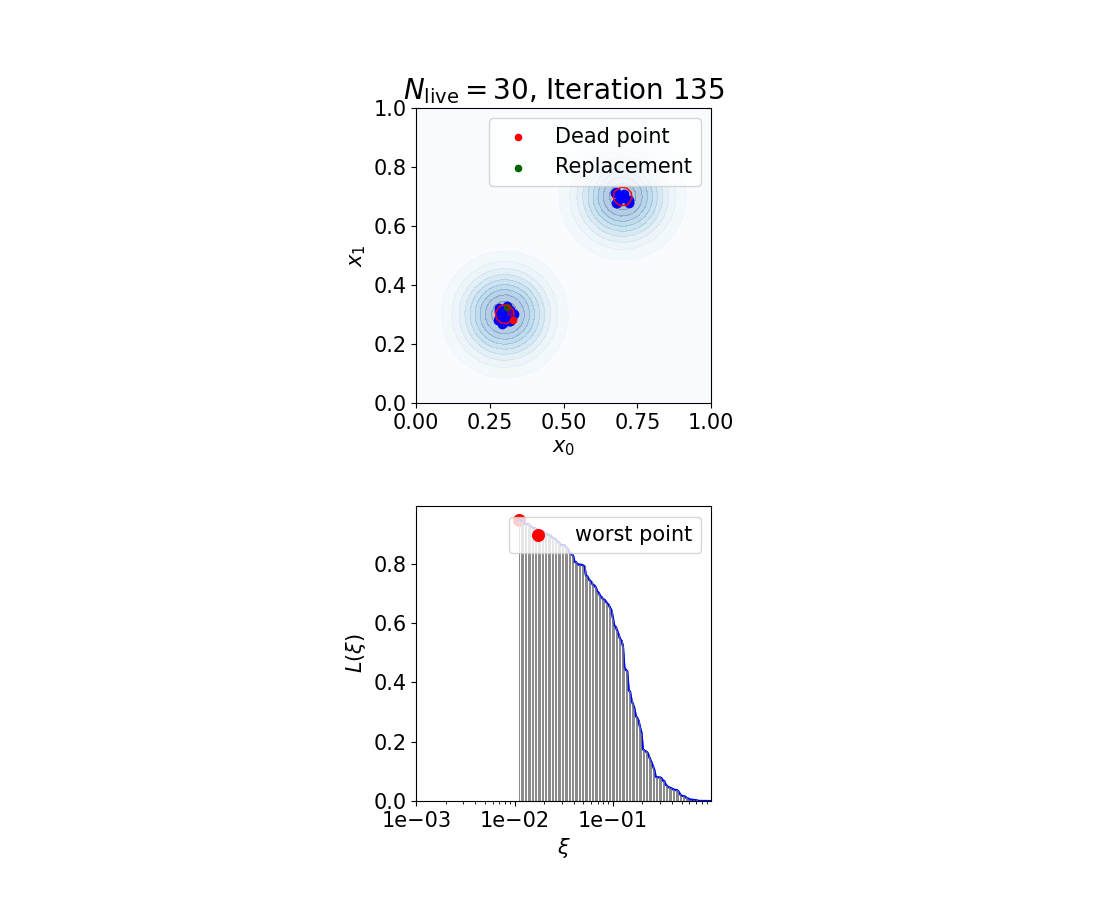
\includegraphics[width=\linewidth,
                             trim=240 20 250 50, clip]{Figures/NS/nested_sampling_135.png}
            }
            \only<8>{
            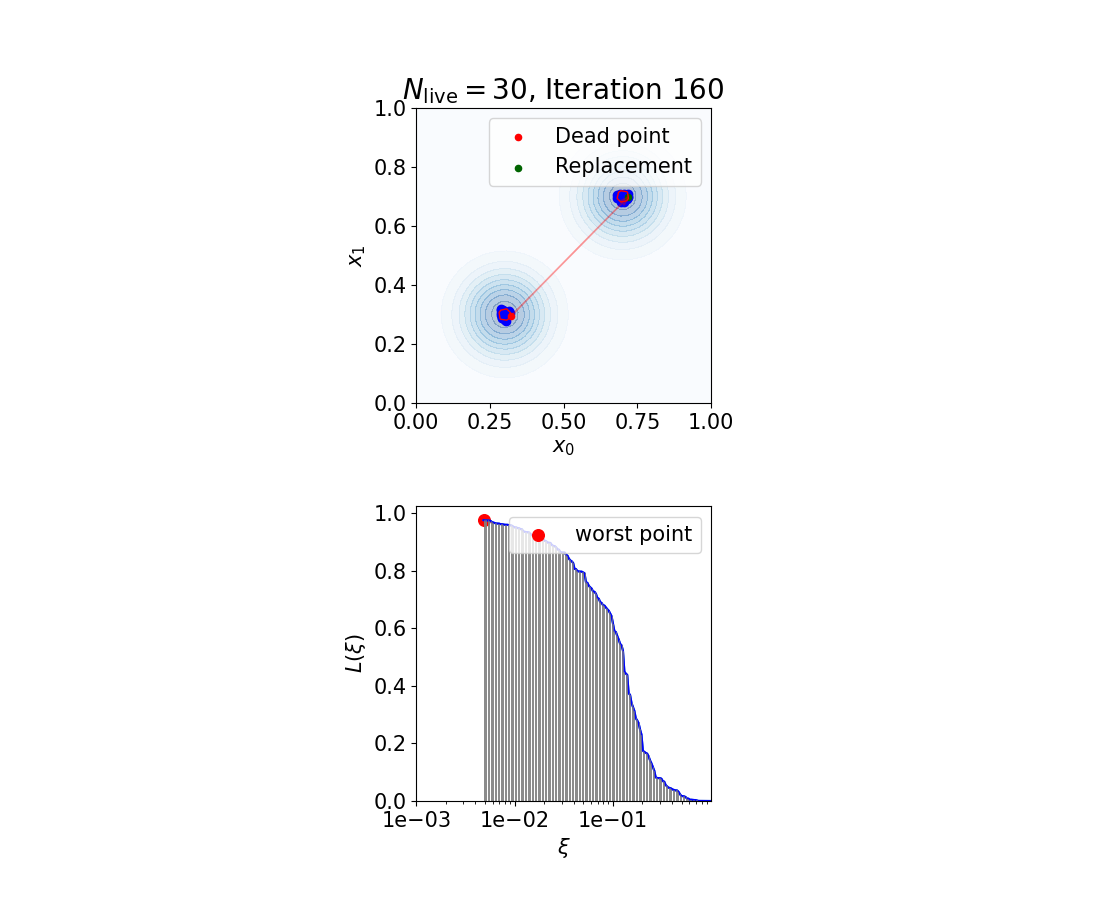
\includegraphics[width=\linewidth,
                             trim=240 20 250 50, clip]{Figures/NS/nested_sampling_160.png}
            }
            \only<9>{
            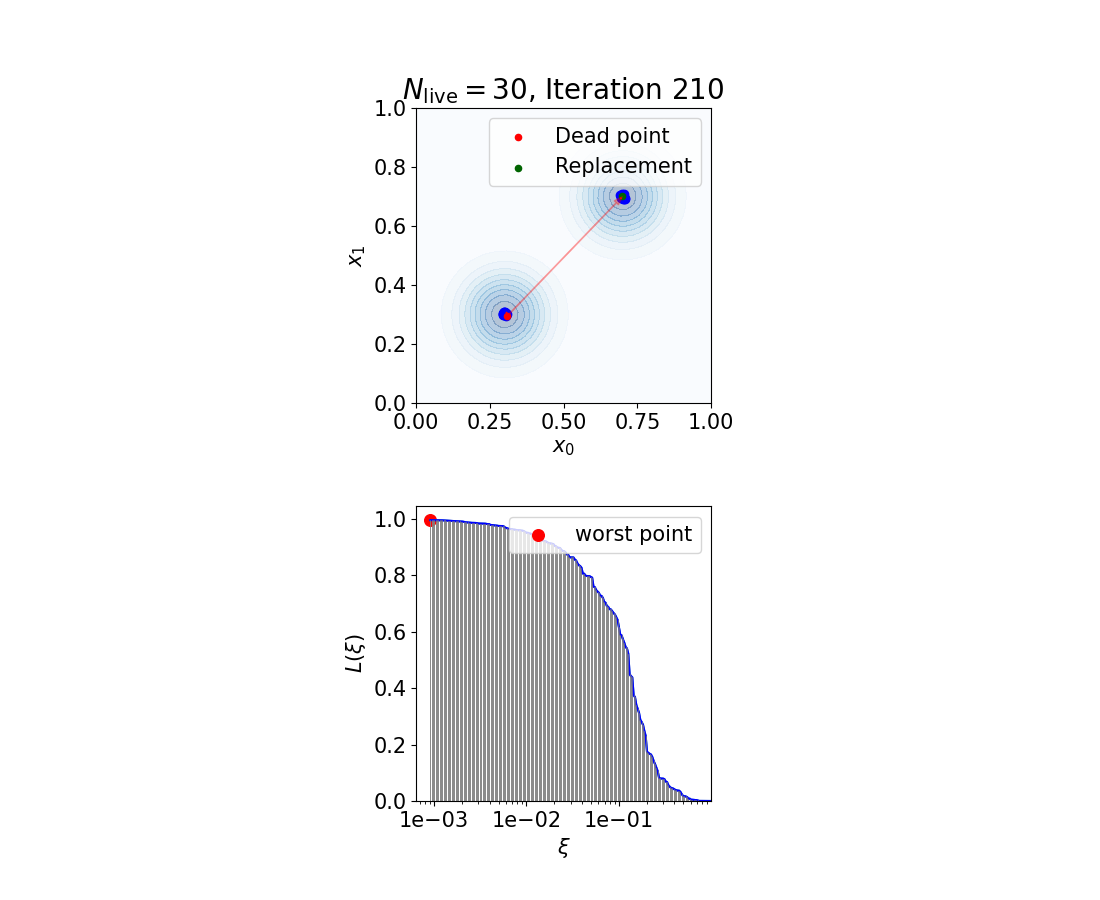
\includegraphics[width=\linewidth,
                             trim=240 20 250 50, clip]{Figures/NS/nested_sampling_210.png}
            }
            \only<10>{
            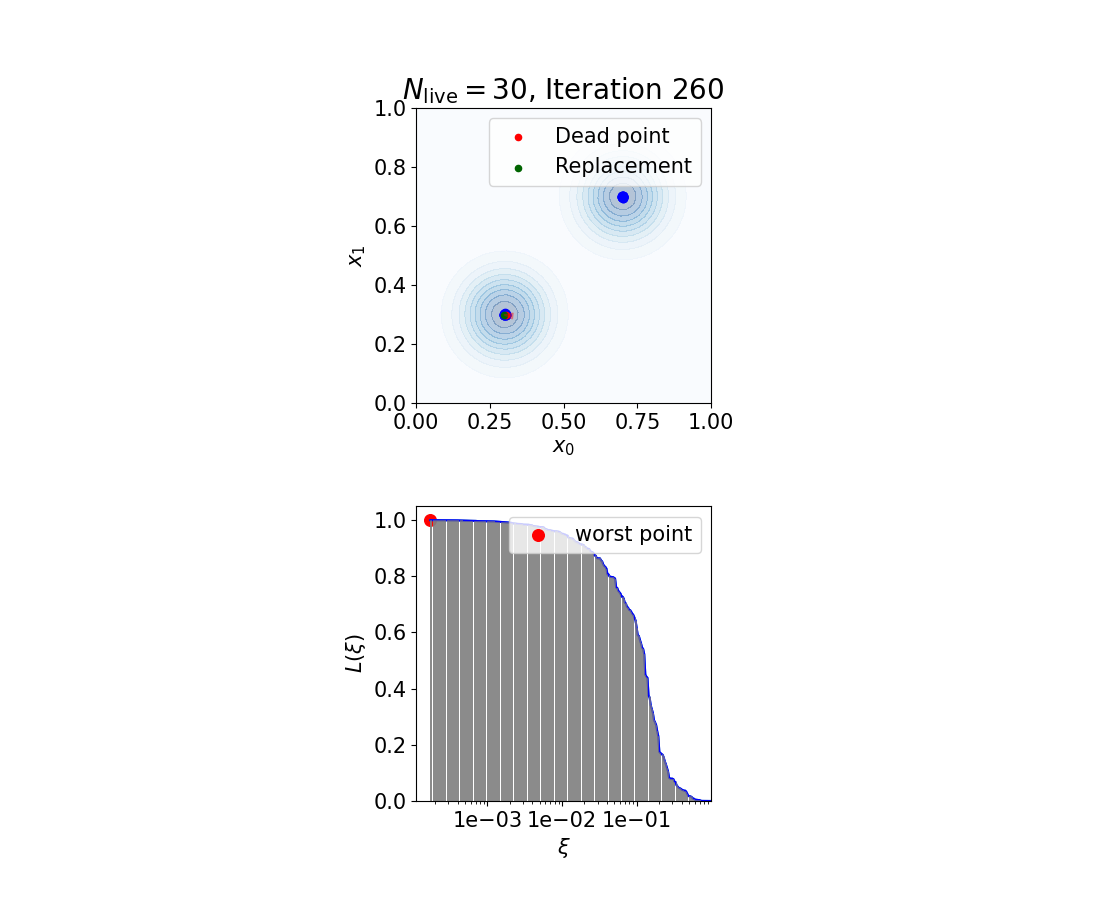
\includegraphics[width=\linewidth,
                             trim=240 20 250 50, clip]{Figures/NS/nested_sampling_260.png}
            }

        \end{figure}
    \end{column}
\end{columns}

\end{frame}

\begin{frame}{Accelerated Nested Sampling}
\vspace{-0.5em}
\begin{columns}
    % ---------- LEFT COLUMN ----------
    \begin{column}{0.60\textwidth}
    \scriptsize
    \textbf{Traditional nested sampling (serial):}
    \begin{itemize}
        \item Remove one `worst' live point each iteration.
        \item New point conditioned on:
        \vspace{-1em}
        $$
        \mathcal{L} > \mathcal{L}_{\min}
        $$
        \item Inherently sequential MCMC slice samples
        \item \texttt{PolyChord - Handley et al 2025}
    \end{itemize}
    \vspace{1em}
    \hline
    \vspace{1em}
    \textbf{Accelerated nested sampling (parallel):}
    \begin{itemize}
        \item Discard a batch of $n_{\text{del}}$ `worst' points.
        \item All replacements conditioned on:
        \vspace{-1em}
        \[
        \mathcal{L}(\theta) > \mathcal{L}_{\min}
        \quad
        \mathcal{L}_{\min} = \max\{\mathcal{L}_1, \ldots, \mathcal{L}_{n_{\text{del}}}\}
        \]
        \item Sample each replacement independently \\ 
              \textcolor{red}{$\Rightarrow$ vectorised (vmap) across GPU}
        \item \texttt{Blackjax}
        \begin{itemize}
        \scriptsize
            \item \texttt{Cabezas at al 2024, Yallup et al 2025}
        \end{itemize} 
    \end{itemize}
 
    \end{column}

    % ---------- RIGHT COLUMN ----------
    \begin{column}{0.325\textwidth}
        \vspace{0.6em}
        \begin{figure}
            \centering

            % ----------- SHOW IMAGE 1 ON OVERLAY 1 -----------
            \only<1>{
            \vspace{-0.7em}
            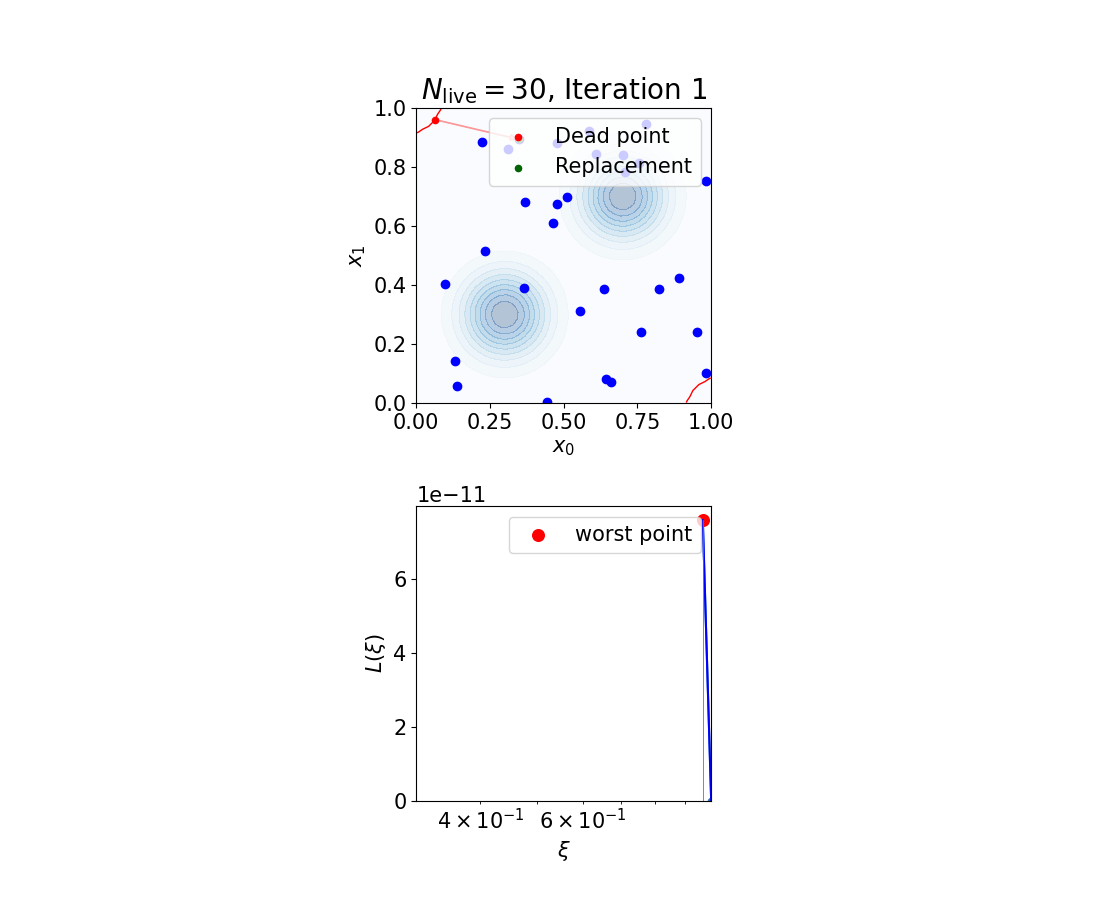
\includegraphics[width=\linewidth,
                             trim=240 300 250 40, clip]{Figures/NS/nested_sampling_1.png}
            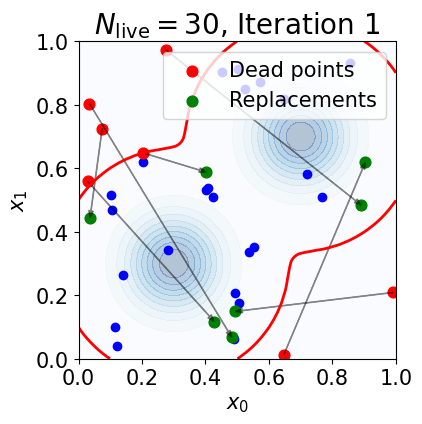
\includegraphics[width=0.9\linewidth]{Figures/NS/parrallel_ns_1.png}
            }

            % ----------- SHOW IMAGE 10 ON OVERLAY 2 -----------
            \only<2>{
            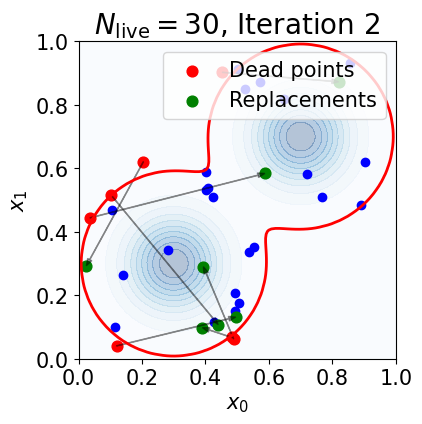
\includegraphics[width=0.9\linewidth]{Figures/NS/parrallel_ns_2.png}
            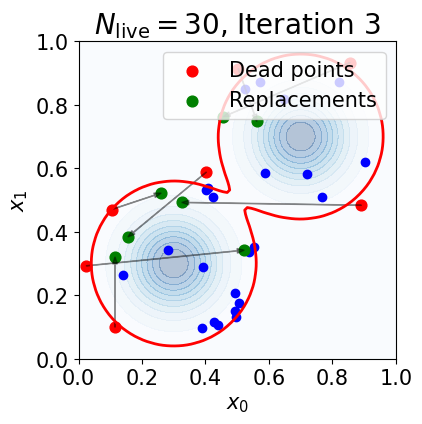
\includegraphics[width=0.9\linewidth]{Figures/NS/parrallel_ns_3.png}
            }

        \end{figure}
    \end{column}
\end{columns}

\end{frame}

\begin{frame}{Benchmarking Nested Sampling}

\textbf{Time Separated Horizon Model Fits}
\scriptsize
\begin{table}[h]
\centering
\renewcommand{\arraystretch}{1.25}
\begin{tabular}{lcccc}
\hline
\textbf{Configuration} &
\textbf{\begin{tabular}{c} Old Time \\ (Hr:Min:Sec) \end{tabular}} &
\textbf{\begin{tabular}{c} New Time \\ (Min:Sec) \end{tabular}} &
\textbf{\begin{tabular}{c} Speed \\ Factor \end{tabular}} &
\textbf{\begin{tabular}{c} Price \\ Factor \end{tabular}} \\
\hline
15 Reg (19 Param) & 12:00:00* & 00:00:49 & 881* & 641* \\
20 Reg (24 Param) & 12:00:00* & 00:02:00 & 360* & 262* \\
35 Reg (39 Param) & 12:00:00* & 00:20:32 & 35*  & 26* \\
\hline
\end{tabular}
\end{table}

{\tiny
* \textcolor{red}{CSD3 timed out prior to completion of fitting - thus lower limits}}

\begin{columns}[T,totalwidth=\textwidth]
    % ---------------- Left Column ----------------
    \begin{column}{0.48\textwidth}
        \centering
        \textbf{NS Parameter Scaling}\\[0.4pt]
        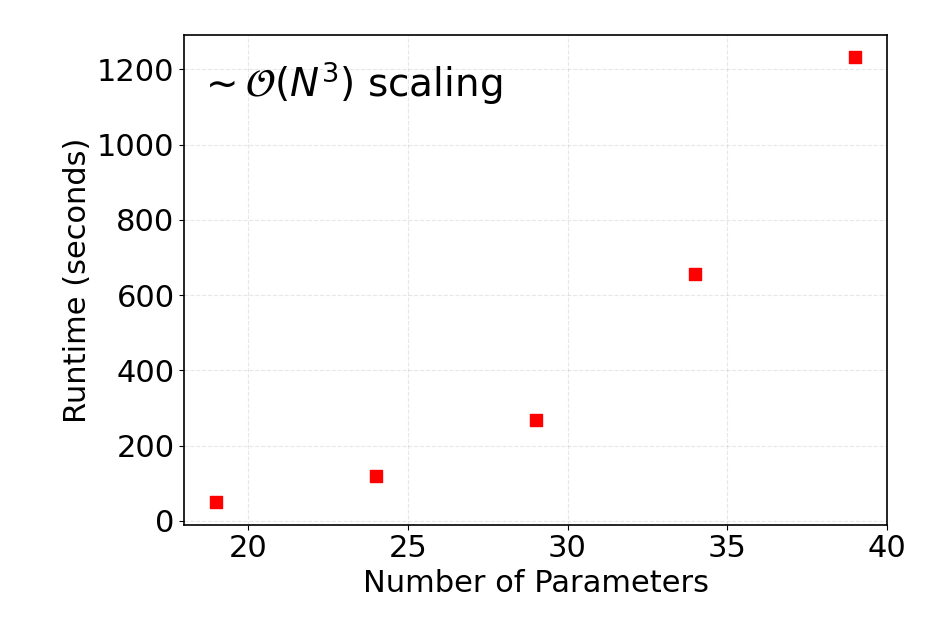
\includegraphics[width=\linewidth]{Figures/ns_scaling.png}
    \end{column}

    % ---------------- Right Column ----------------
    \begin{column}{0.48\textwidth}
        \centering
        \textbf{Signal Recovery}\\[0.4pt]
        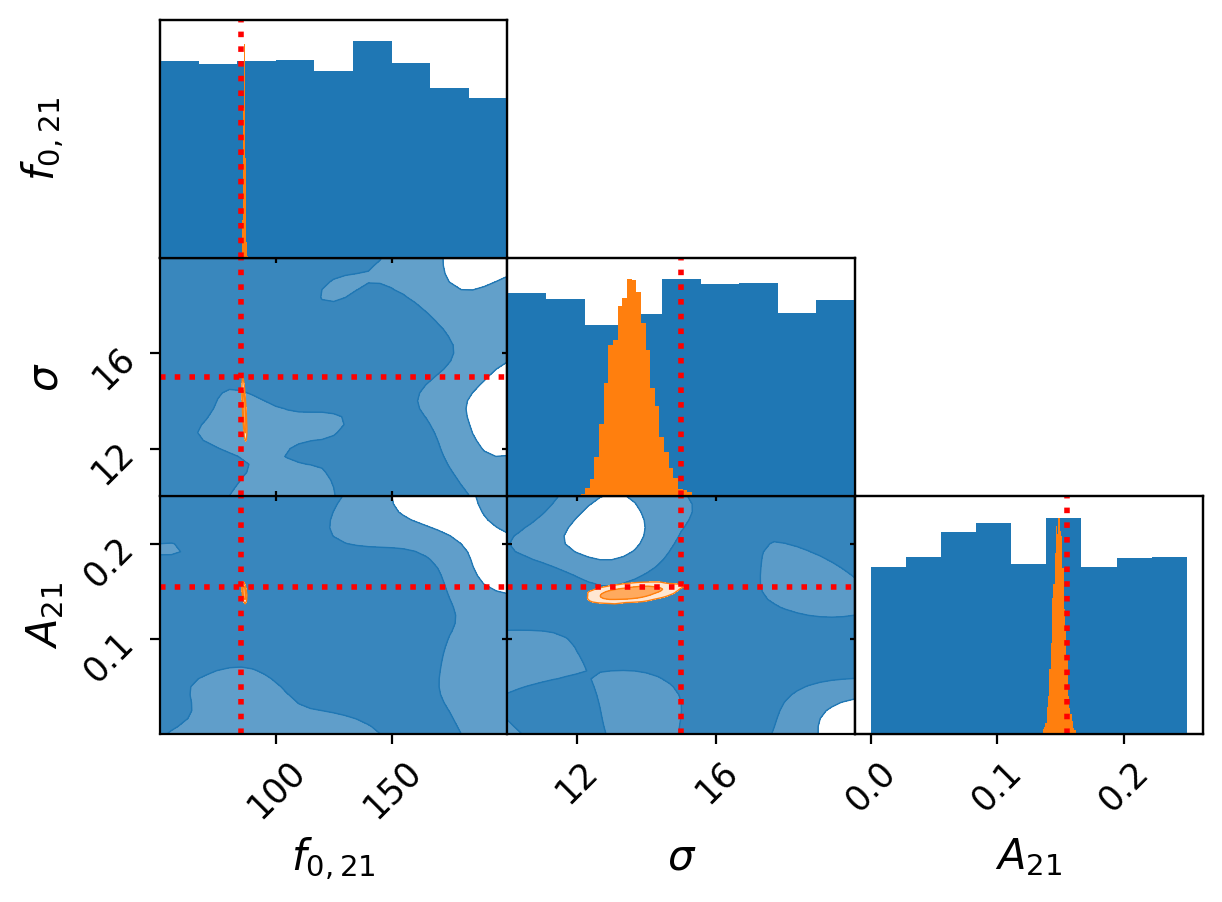
\includegraphics[width=0.8\linewidth]{Figures/signal_corner.png}
        \vspace{-0.8em}
        {\tiny
        * Time-Separated, Gaussian Signal, 20 Region, No Horizon
        }
    \end{column}
\end{columns}

\end{frame}



\begin{frame}{Future of REACH Pipeline?}
\textbf{Accelerated Forward Model:}
\footnotesize

\[
\boldsymbol{
T_{\mathrm{obs}}(\nu)
=
T_{21}(\nu)
+ T_{\mathrm{FG}}(\nu)
+ \sigma(\nu)
}
\]


\footnotesize
\begin{table}[h]
\centering
\begin{tabular}{l c}
\hline
\textbf{Configuration} & \textbf{New (ms)} \\
\hline
Ave No Horizon      & 0.59 \\
Ave Horizon         & 0.63 \\
Sep No Horizon     & 0.61 \\
Sep Horizon        & 0.59 \\
\hline
\end{tabular}
\end{table}

\vspace{-0.5em}

{\tiny
\emph{
\hspace{17em} * Averaged over 1000 forward model calls \\
\hspace{17em} * Run on an NVIDIA A100 GPU (\pounds 0.55/hr) \\
\hspace{17em} * Gaussian signal and noise structure\\
}
}


\scriptsize
\textbf{Note:} An order of magnitude faster without noise addition.
\pause
\small 

\vspace{1em}

\textbf{Future of REACH Simulations}
\begin{itemize}
    \item XLA compilation and full vectorisation / parallelisation allows:
    \vspace{-0.5em}
    \[
    \boldsymbol{
        \textcolor{red}{
        \mathcal{O}(10^6)\ \text{simulations per second}}}
    \]
\end{itemize}

\end{frame}

\begin{frame}{Future of REACH Pipeline?}
\textbf{Simulation Based Inference}\\[6pt]

\footnotesize
As we begin to consider more parameterisations of our system
\begin{itemize}
    \item eg. Parameterised/ Emulated Beam Pattern (+4/5)
    \item Saxena et al 2024 - TMNRE 
\end{itemize}
\centering

\only<1>{
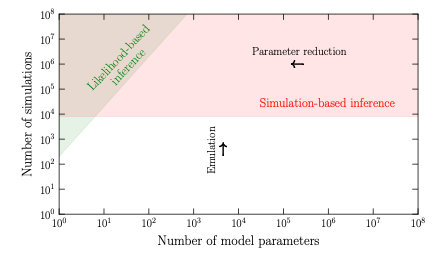
\includegraphics[width=0.7\linewidth]{Figures/scaling_sbi.png}

\vfill

\hfill \tiny Boddy et al 2022
}

\end{frame}



\begin{frame}{Questions}
\centering
\vspace{1em}
\textbf{Thank you for your attention!}
\vspace{1.5em}
\begin{minipage}{0.8\textwidth}
\centering
\footnotesize
\textbf{Jacob Tutt} \\
Department of Physics, University of Cambridge \\
\texttt{jlt67@cam.ac.uk} \\
\faGithub\ \href{https://github.com/REACH-telescope/REACH_data_analysis_gpu}{REACH-telescope/REACH\_data\_analysis\_gpu}
\end{minipage}
\end{frame}




\begin{frame}{An Introduction to JAX}
\footnotesize
% ---------------- TOP BAR ----------------
\begin{columns}[T,totalwidth=\textwidth]

% ---- LEFT: JAX logo + subtitle ----
\begin{column}{0.28\textwidth}
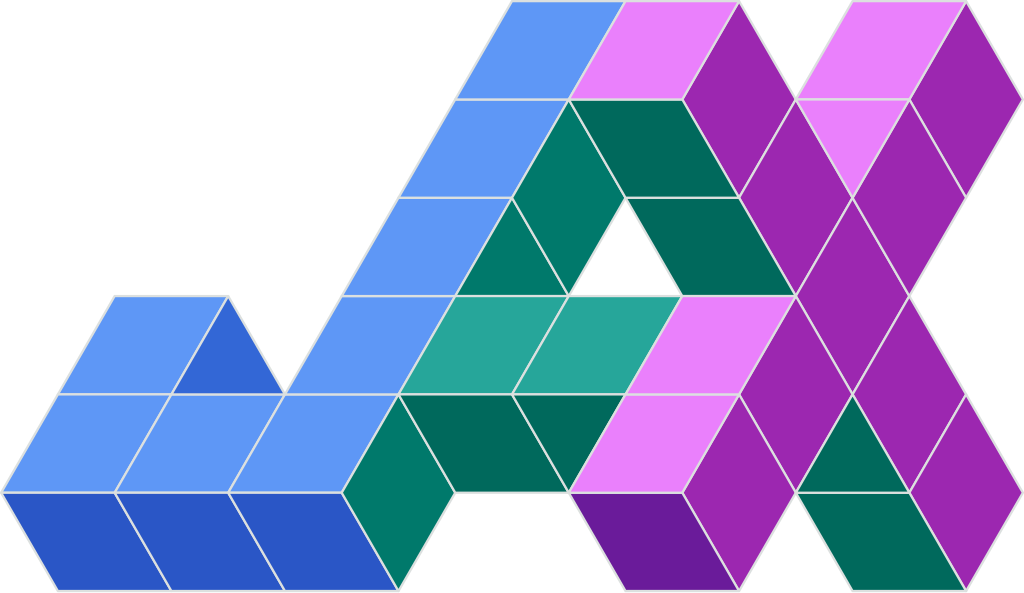
\includegraphics[width=0.75\linewidth]{Figures/jax.png}

\vspace{0.2em}
\footnotesize
\textbf{High-performance numerical-computing}\\
\textbf{and large-scale machine learning}
\end{column}

\begin{column}{0.715\textwidth}
\vspace{-1.6em}
\begin{block}{Automatic Differentiation}
\small
Provides `free' exact derivatives of numerical at machine precision by systematically applying the chain rule. 
\vspace{-1.5em}
\[
(\nabla f)(x)_i = \frac{\partial f}{\partial x_i}(x)
\quad\Longrightarrow\quad 
\texttt{jax.grad(f)(x)}
\]
\scriptsize For more details on Autodiff/Dual Numbers see \\ \faGithub\ \href{https://github.com/JacobTutt/dual_autodiff_package}{JacobTutt/dual\_autodiff\_package}

\end{block}
\end{column}

\end{columns}

% ---------------- SECTION DIVIDER ----------------


% -------------- BOTTOM: TWO APPLICATIONS ----------------
\begin{columns}[T,totalwidth=\textwidth]
% ---- LEFT: Optax / optimisation ----
\begin{column}{0.46\textwidth}
\begin{block}{Gradient-based Optimisation}
\scriptsize
JAX computes gradients of a loss function:
\vspace{-0.6em}
\[
\nabla_\theta \, \mathcal{L}(\theta) = \texttt{jax.grad}(\mathcal{L})(\theta)
\]
\vspace{-0.3em}
Exploited during ML training's gradient descent loops using \textbf{Optax}'s optimisers (e.g. Adam):
\begin{columns}
\begin{column}{0.7\textwidth}
\vspace{-0.3em}
\[
\theta_{t+1} = \theta_t - \alpha \, \frac{m_t}{\sqrt{v_t} + \epsilon}
\]
\end{column}
\begin{column}{0.28\textwidth}
\vspace{-1.3em}

\includegraphics[width=0.7\linewidth]{Figures/optax.png}
\end{column}
\end{columns}
\vspace{-0.2em}
\end{block}

\end{column}

% ---- RIGHT: BlackJAX / HMC ----
\begin{column}{0.51\textwidth}
\begin{block}{Hamiltonian Monte Carlo/ NUTS}
\scriptsize
Exploits gradients of the log-posterior to accelerate exploration of parameter space:
\vspace{-0.3em}
\[
\nabla_\theta \log p(\theta \mid D)
\]
\vspace{-0.3em}
\textbf{BlackJAX} enables efficient sampler implementations (eg via Leapfrog Integration).
\begin{columns}
\begin{column}{0.7\textwidth}
\[
(p, q) \longrightarrow (p', q') \quad 
\]
\end{column}
\begin{column}{0.28\textwidth}


\includegraphics[width=0.5\linewidth]{Figures/blackjax.jpeg}
\end{column}
\end{columns}
\vspace{-0.2em}
\end{block}

\end{column}

\end{columns}

\end{frame}


\begin{frame}{An Introduction to JAX}
\footnotesize

% ---------------- TOP BAR ----------------
\begin{columns}[T,totalwidth=\textwidth]

% ---- LEFT: JAX logo + subtitle ----
\begin{column}{0.28\textwidth}
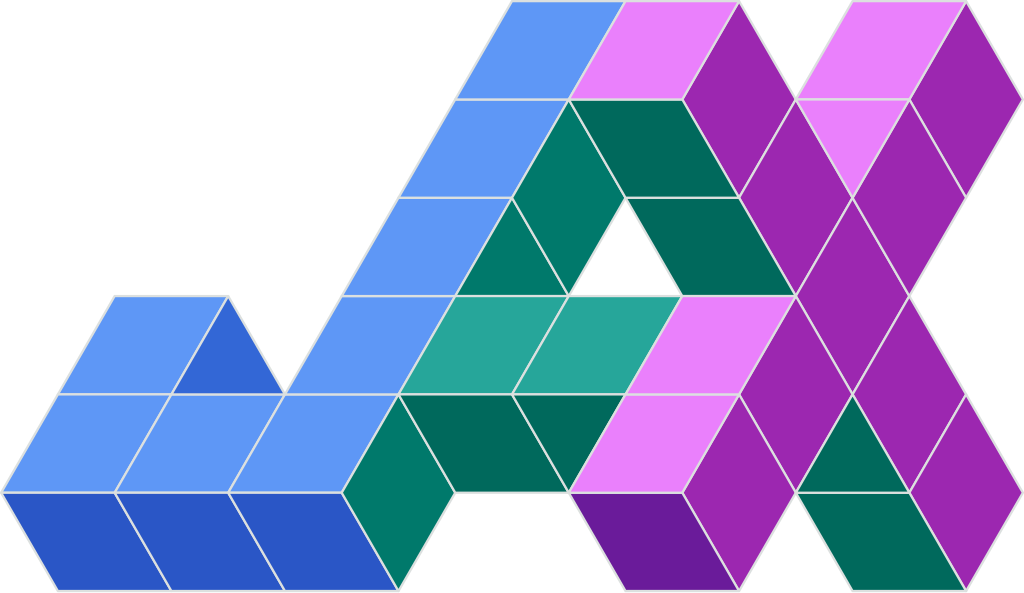
\includegraphics[width=0.75\linewidth]{Figures/jax.png}

\vspace{0.2em}
\footnotesize
\textbf{High-performance numerical-computing}\\
\textbf{and large-scale machine learning}
\end{column}

% ---- RIGHT: XLA + JIT explanation ----
\begin{column}{0.715\textwidth}
\vspace{-1.6em}
\begin{block}{XLA Compilation}
\small
Transforms functions into optimised machine code:
\scriptsize
\begin{itemize}
    \item Inputs are wrapped in \emph{tracers}
    \item JAX operation mapped to a computation graph (intermediate).
    \item jaxpr then device-dependently XLA compiled
\end{itemize}

\vspace{-1em}
\[
f(x) \quad\Longrightarrow\quad \texttt{jax.jit}(f)(x)
\]
\end{block}
\end{column}

\end{columns}

% ---------------- BOTTOM ----------------
\vspace{0.3em}
\begin{columns}[T,totalwidth=\textwidth]
% ---- LEFT: Compiled vs Interpreted ----
\begin{column}{0.46\textwidth}
\begin{block}{Compiled Languages}
\scriptsize
\begin{itemize}
    \item Ahead-of-time compilation to machine code
    \item Static typing and memory layout
    \item Highly optimised loops / vectorisation
\end{itemize}
\vspace{0.2em}
\textbf{Pros:} low-level control, maximum hardware efficiency.
\end{block}
\end{column}

% ---- RIGHT: How JAX Bridges the Gap ----
\begin{column}{0.51\textwidth}
\begin{block}{Python + Compiled Speed}
\scriptsize
\begin{itemize}
    \item Python - slow interpreted language.
    \item Produces near-C++ speeds
    \item Supports GPUs with little code changes
\end{itemize}
\vspace{1.3em}
\textbf{JAX provides Python's flexibility with compiled-language performance.}
\end{block}
\end{column}
\end{columns}
\end{frame}

\begin{frame}[fragile]{An Introduction to JAX}
\footnotesize

% ---------------- TOP BAR ----------------
\begin{columns}[T,totalwidth=\textwidth]

% ---- LEFT: JAX LOGO ----
\begin{column}{0.28\textwidth}
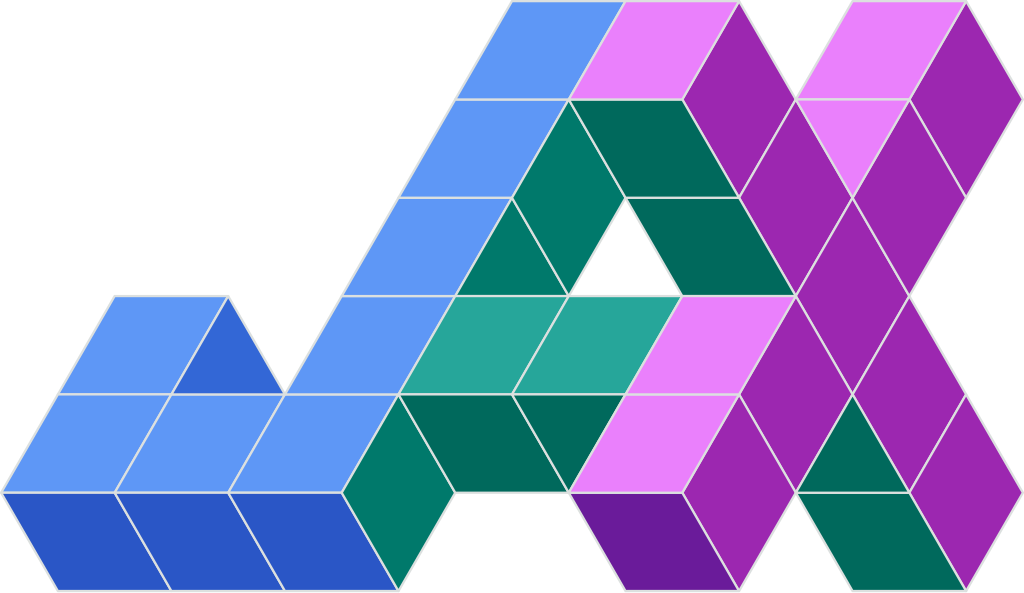
\includegraphics[width=0.75\linewidth]{Figures/jax.png}

\vspace{0.2em}
\footnotesize
\textbf{High-performance numerical-computing}\\
\textbf{and large-scale machine learning}
\end{column}

% ---- RIGHT: VMAP / PMAP OVERVIEW ----
\begin{column}{0.715\textwidth}
\vspace{-1.6em}
\begin{block}{Automatic Vectorisation and Parallelisation}
\small
\vspace{-0.5em}
\begin{itemize}\scriptsize
    \item \textbf{\texttt{jax.vmap}}: automatic vectorisation over batches of data  
    \begin{itemize}\scriptsize
    \item Deals with batches inside primitive operations
    \end{itemize}
    \item \textbf{\texttt{jax.pmap}}: parallel execution across multiple XLA devices  
    \begin{itemize}\scriptsize
    \item True hardware-level parallelism (SPMD)
    \end{itemize}
\end{itemize}

\vspace{-2em}
\[
f(x) \;\Longrightarrow\; \texttt{vmap}(f)(X)
\qquad\qquad
f(x) \;\Longrightarrow\; \texttt{pmap}(f)(X)
\]
\vspace{-2em}
\end{block}
\end{column}

\end{columns}

% ---------------- BOTTOM SECTION ----------------
\vspace{0.3em}

\begin{columns}[T,totalwidth=\textwidth]

% ---------- LEFT: VMAP ----------
\begin{column}{0.48\textwidth}
\begin{block}{From Loops to Vectorisation}
\scriptsize

\textbf{Old way (NumPy/Python):}
\vspace{-0.5em}
\begin{verbatim}
outputs = []
for i in range(N):
    outputs.append(f(xs[i]))
\end{verbatim}
\vspace{-0.5em}
\textbf{New way (JAX):}
\vspace{-0.5em}
\[
\texttt{vmap}(f)(x_{1:N})
\]
\vspace{-1.5em}
\end{block}
\end{column}

% ---------- RIGHT: PMAP ----------
\begin{column}{0.48\textwidth}
\begin{block}{CPU to GPU Parallelism}
\scriptsize

\textbf{Old way (MPI / multi-CPU):}

\begin{verbatim}
with ProcessPoolExecutor() as ex:
    results = list(ex.map(f, xs))
\end{verbatim}

\textbf{New way (JAX):}
\vspace{-0.5em}
\[
\texttt{pmap}(f)(x_{\text{devices}})
\]
\end{block}
\end{column}
\end{columns}
\end{frame}



\end{document}


